\section{Materials and where they come from}
Over 99\% of a ring's mass is lunar: about 320\,Mt once interior decks are counted (the $\sim$300\,Mt used elsewhere leaves them out). Earth supplies the precise fraction of a per cent: electronics, machines, batteries, biology and, unless asteroids or polar ice deliver it, nitrogen.

\begin{figure}[H]
  \centering
  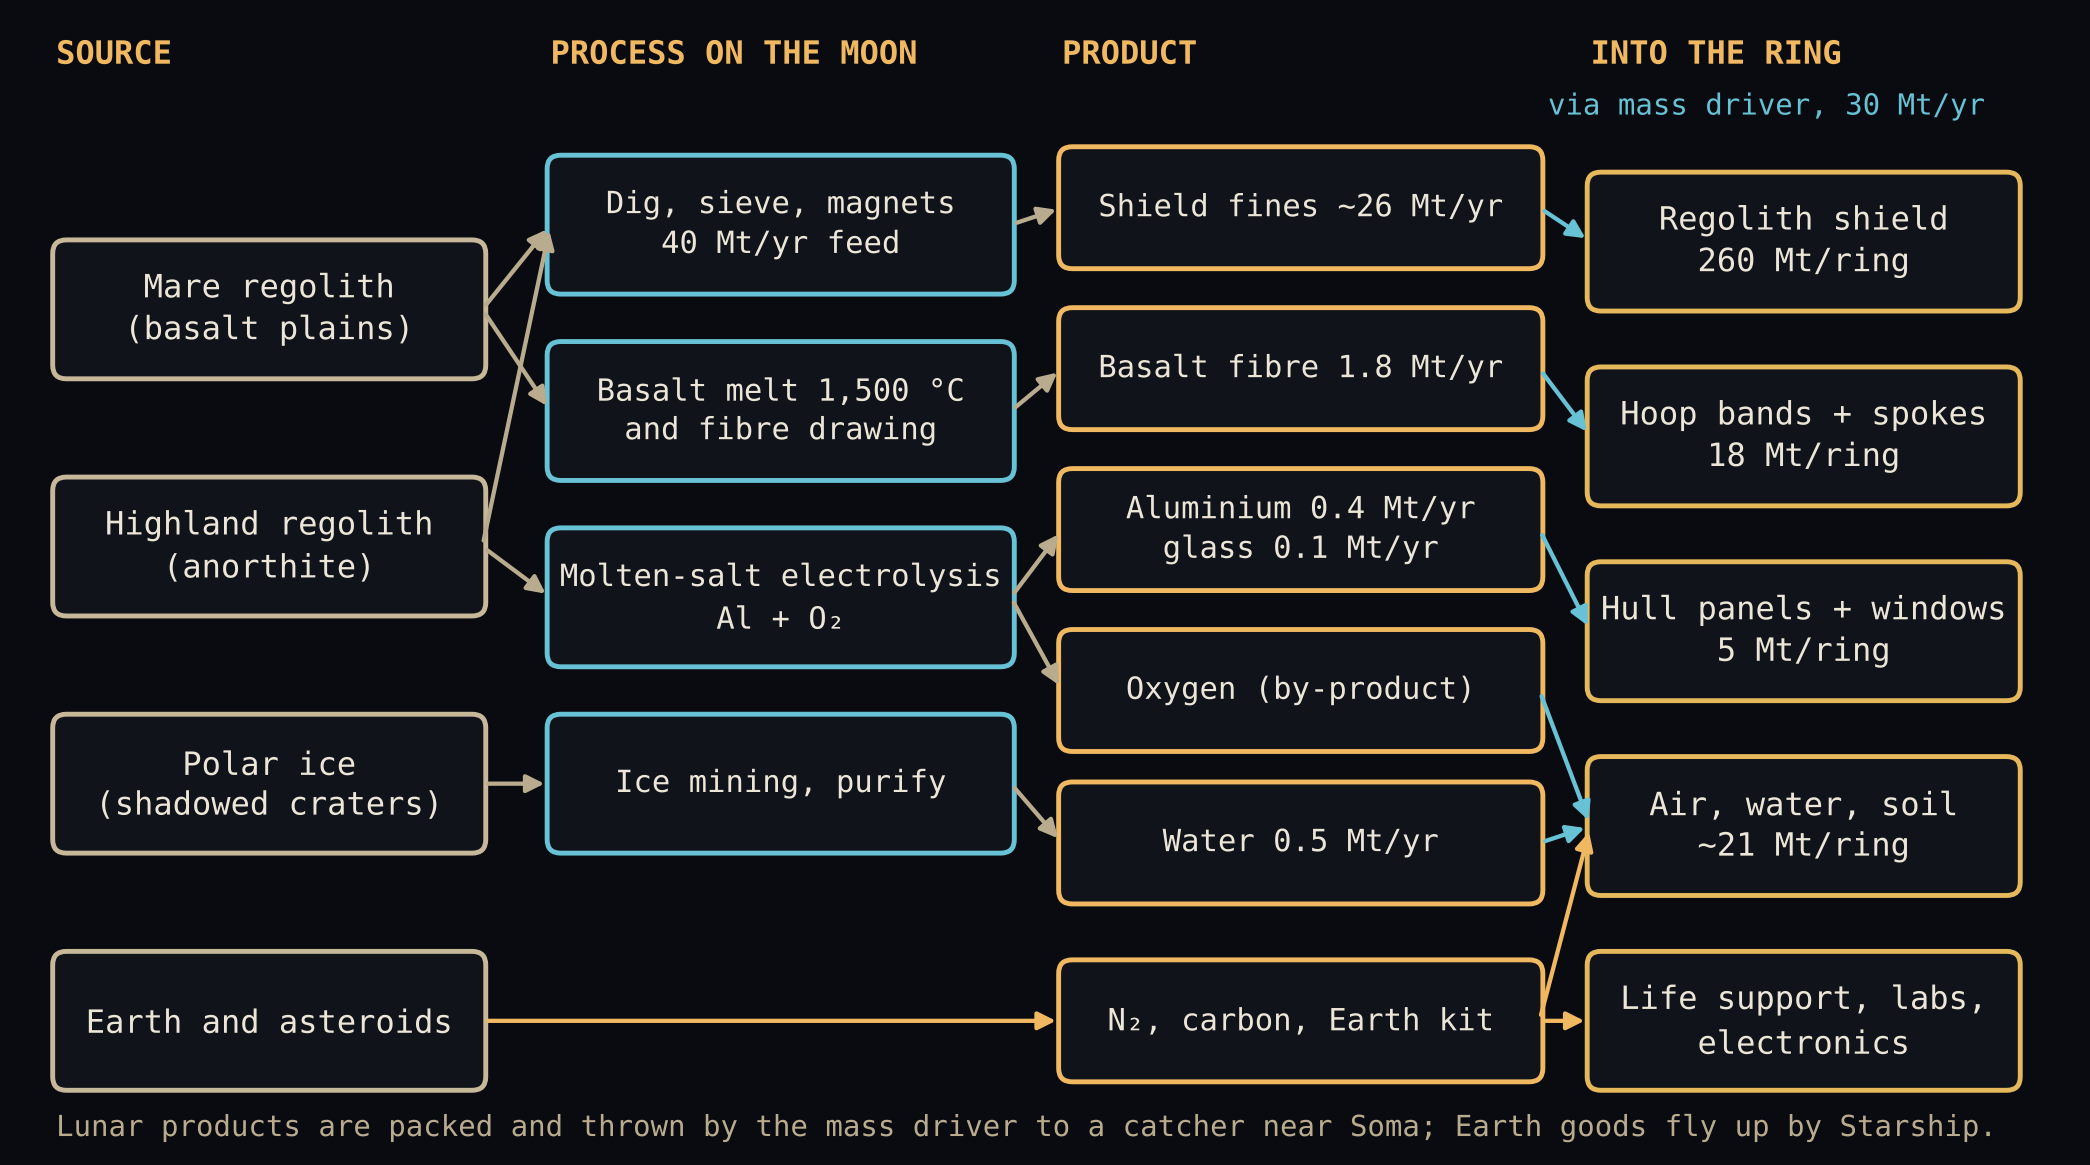
\includegraphics[width=\textwidth]{figures/material_flow.png}
  \caption{Material flow from lunar and Earth sources to the ring. Lunar products are packed and thrown by the mass driver; Earth goods fly up by Starship.}
\end{figure}

\begin{table}[H]
  \centering\small
  \begin{tabularx}{\textwidth}{@{}lrXX@{}}
    \toprule
    \textbf{Material} & \textbf{Per ring} & \textbf{Source} & \textbf{Process} \\
    \midrule
    Regolith shield & 260\,Mt & Mare and highland surface regolith & Dug, sieved, packed into bags; never spins \\
    Basalt fibre (hoops, spokes) & 18\,Mt & Mare basalt & Melted at 1,500\,\textdegree C, drawn through bushings, wound into bands \\
    Aluminium (hull, decks) & 4\,Mt & Highland anorthite & Molten-salt electrolysis; oxygen is a by-product \\
    Glass (windows) & 1\,Mt & Regolith silica & Melted and float-formed on the Moon \\
    Decks and frames & 15\,Mt & Aluminium, basalt composite, sintered regolith & Pressed panels and printed blocks \\
    Soil & 15\,Mt & Sieved regolith + carbon & Carbon from C-type asteroids or Earth; inoculated with soil biology from Earth \\
    Water & 5\,Mt & Polar ice in shadowed craters & Mined, melted, purified \\
    Oxygen & 0.5\,Mt & Regolith oxides & By-product of aluminium and oxygen extraction \\
    Nitrogen & 0.3--0.6\,Mt & Earth today; asteroids or polar volatiles later & Shipped as liquid; the main open supply question \\
    Earth high-tech kit & 50,000\,t & Earth & Electronics, life-support machines, lab gear, seeds and microbes \\
    Batteries & 37,500\,t & Earth & 6\,GWh of storage for spin-up, eclipses and peaks \\
    \bottomrule
  \end{tabularx}
  \caption{Bill of materials for one ring, with sources.}
\end{table}

\begin{figure}[H]
  \centering
  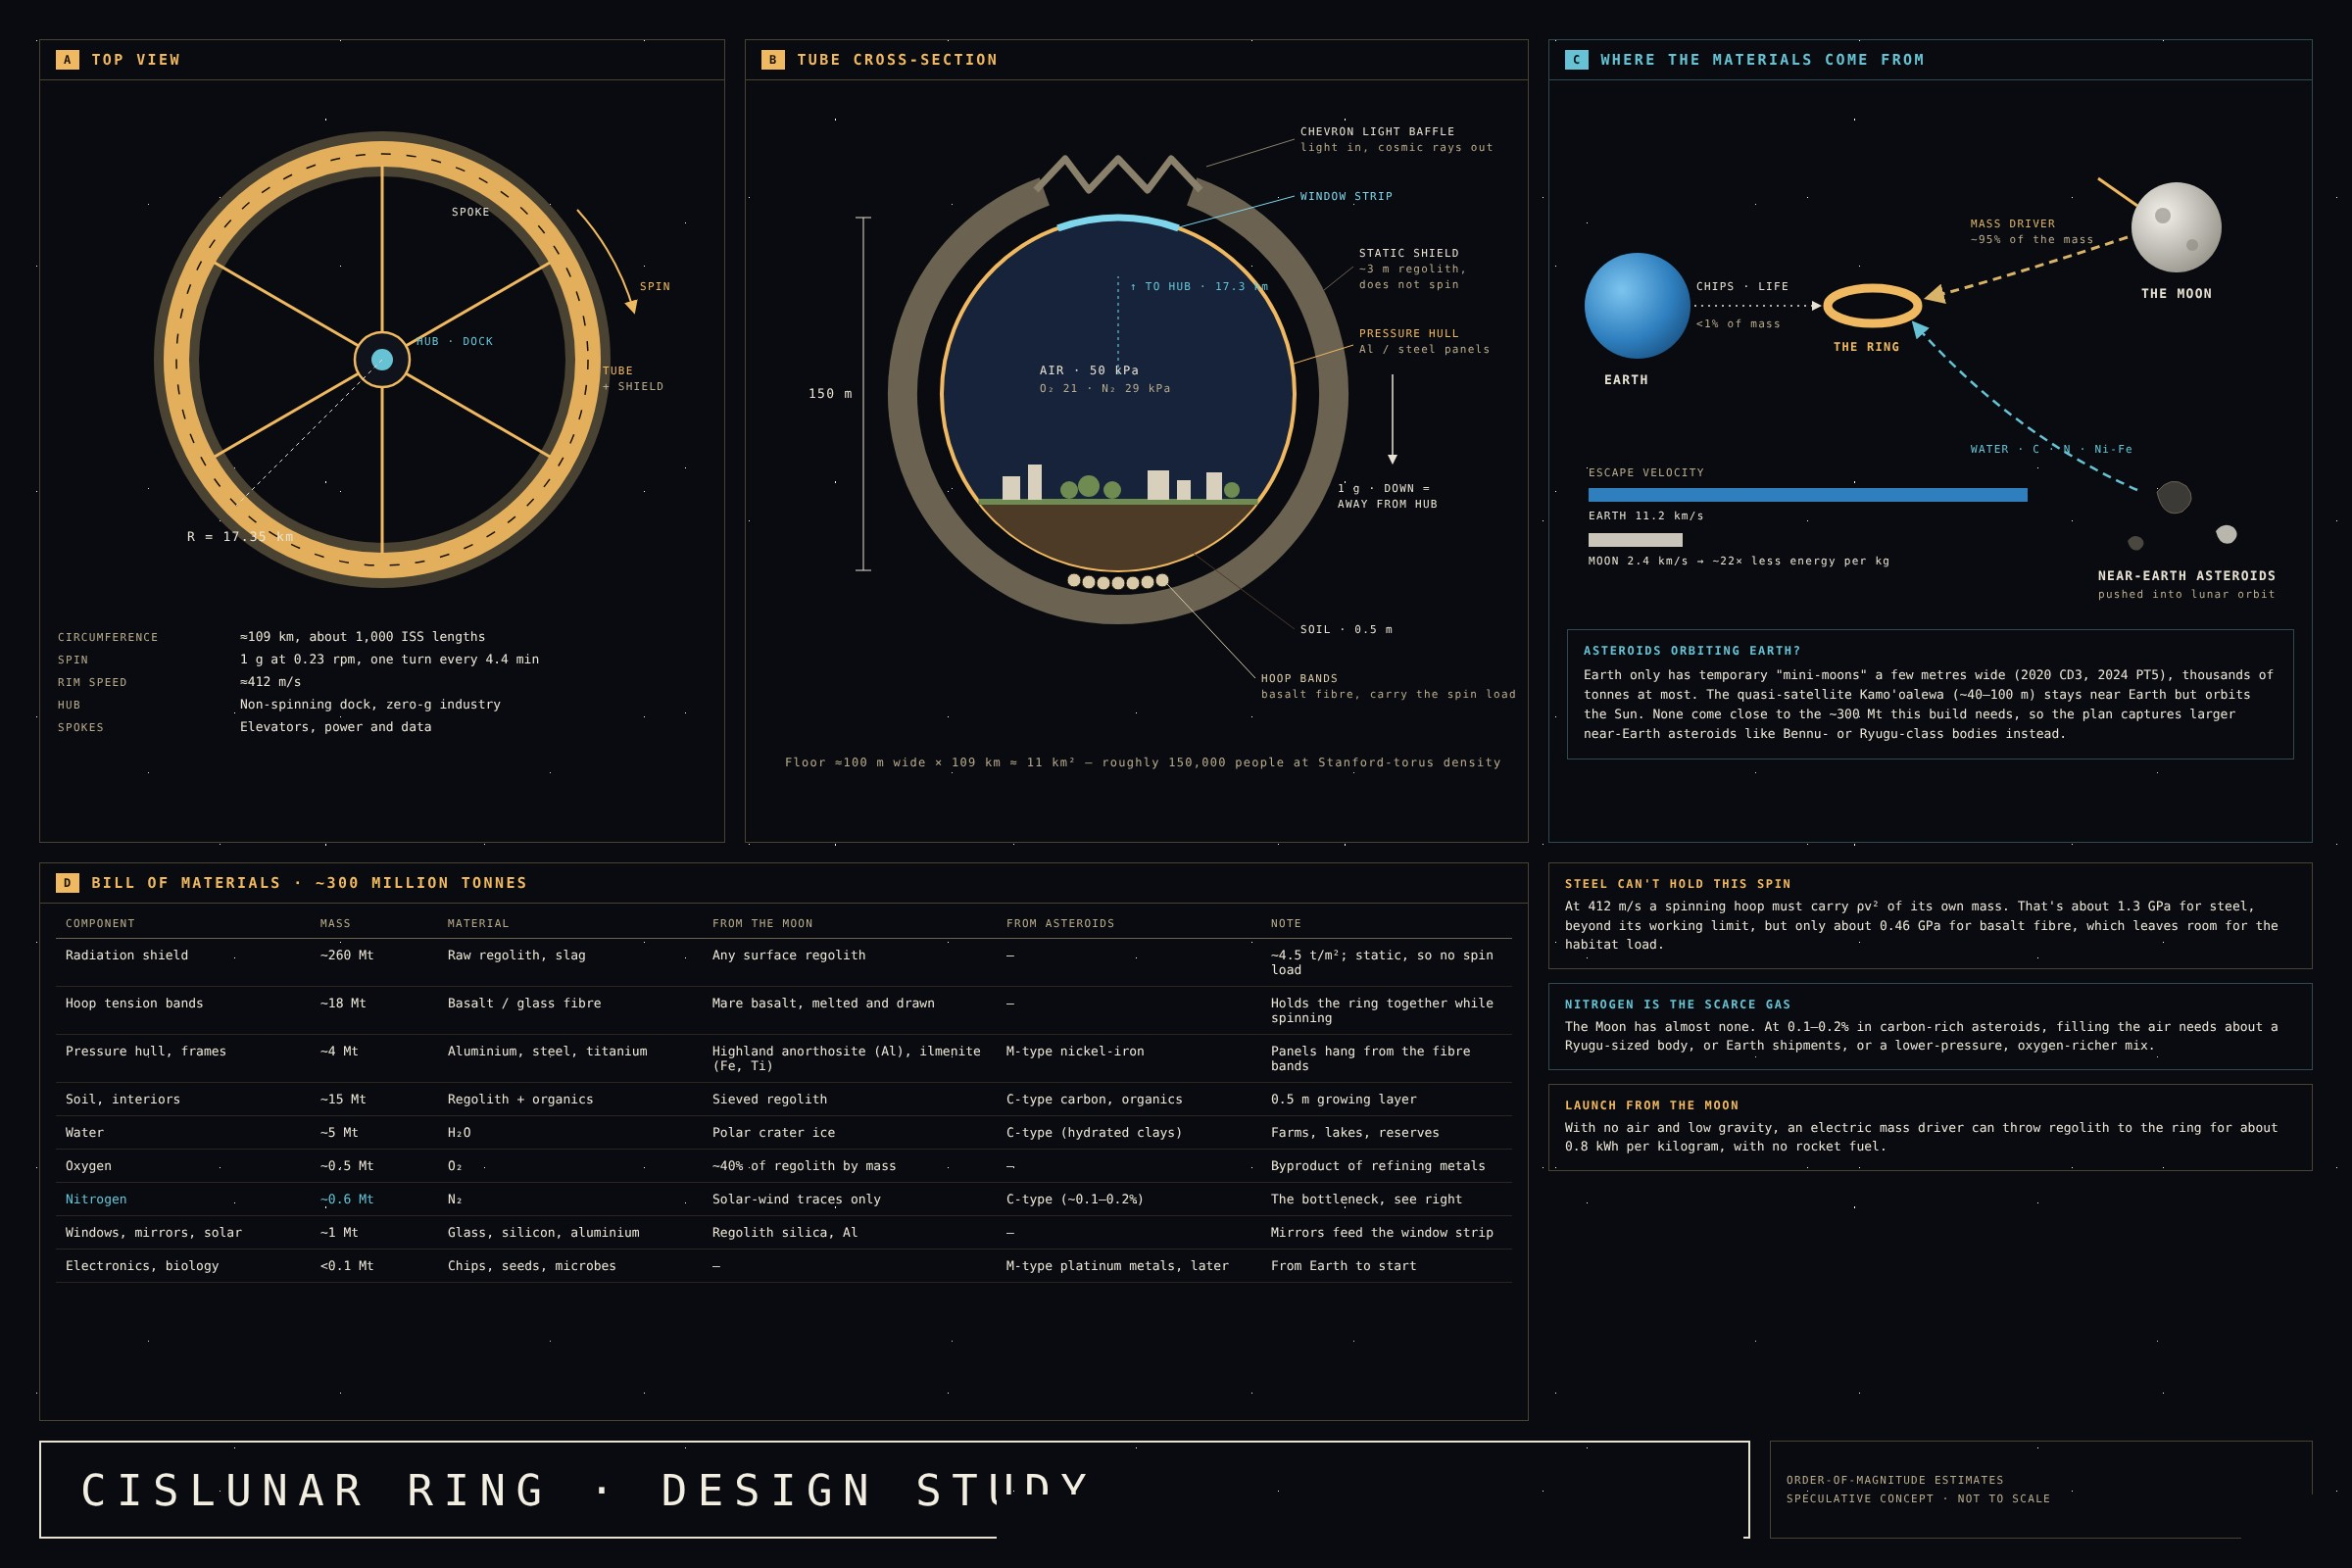
\includegraphics[width=\textwidth]{figures/board-cislunar-ring-design.jpg}
  \caption{Design board: the ring, its 150\,m tube, the static regolith shield and the bill of materials.}
\end{figure}

\section{Materials and cost by cell type}
A ring has 606 cells of 180\,m, in 11 types. Every cell carries the same shell ($\sim$465\,kt of shield, hoop bands, hull and glass); what differs is the interior and the Earth-made kit inside it.

\begin{figure}[H]
  \centering
  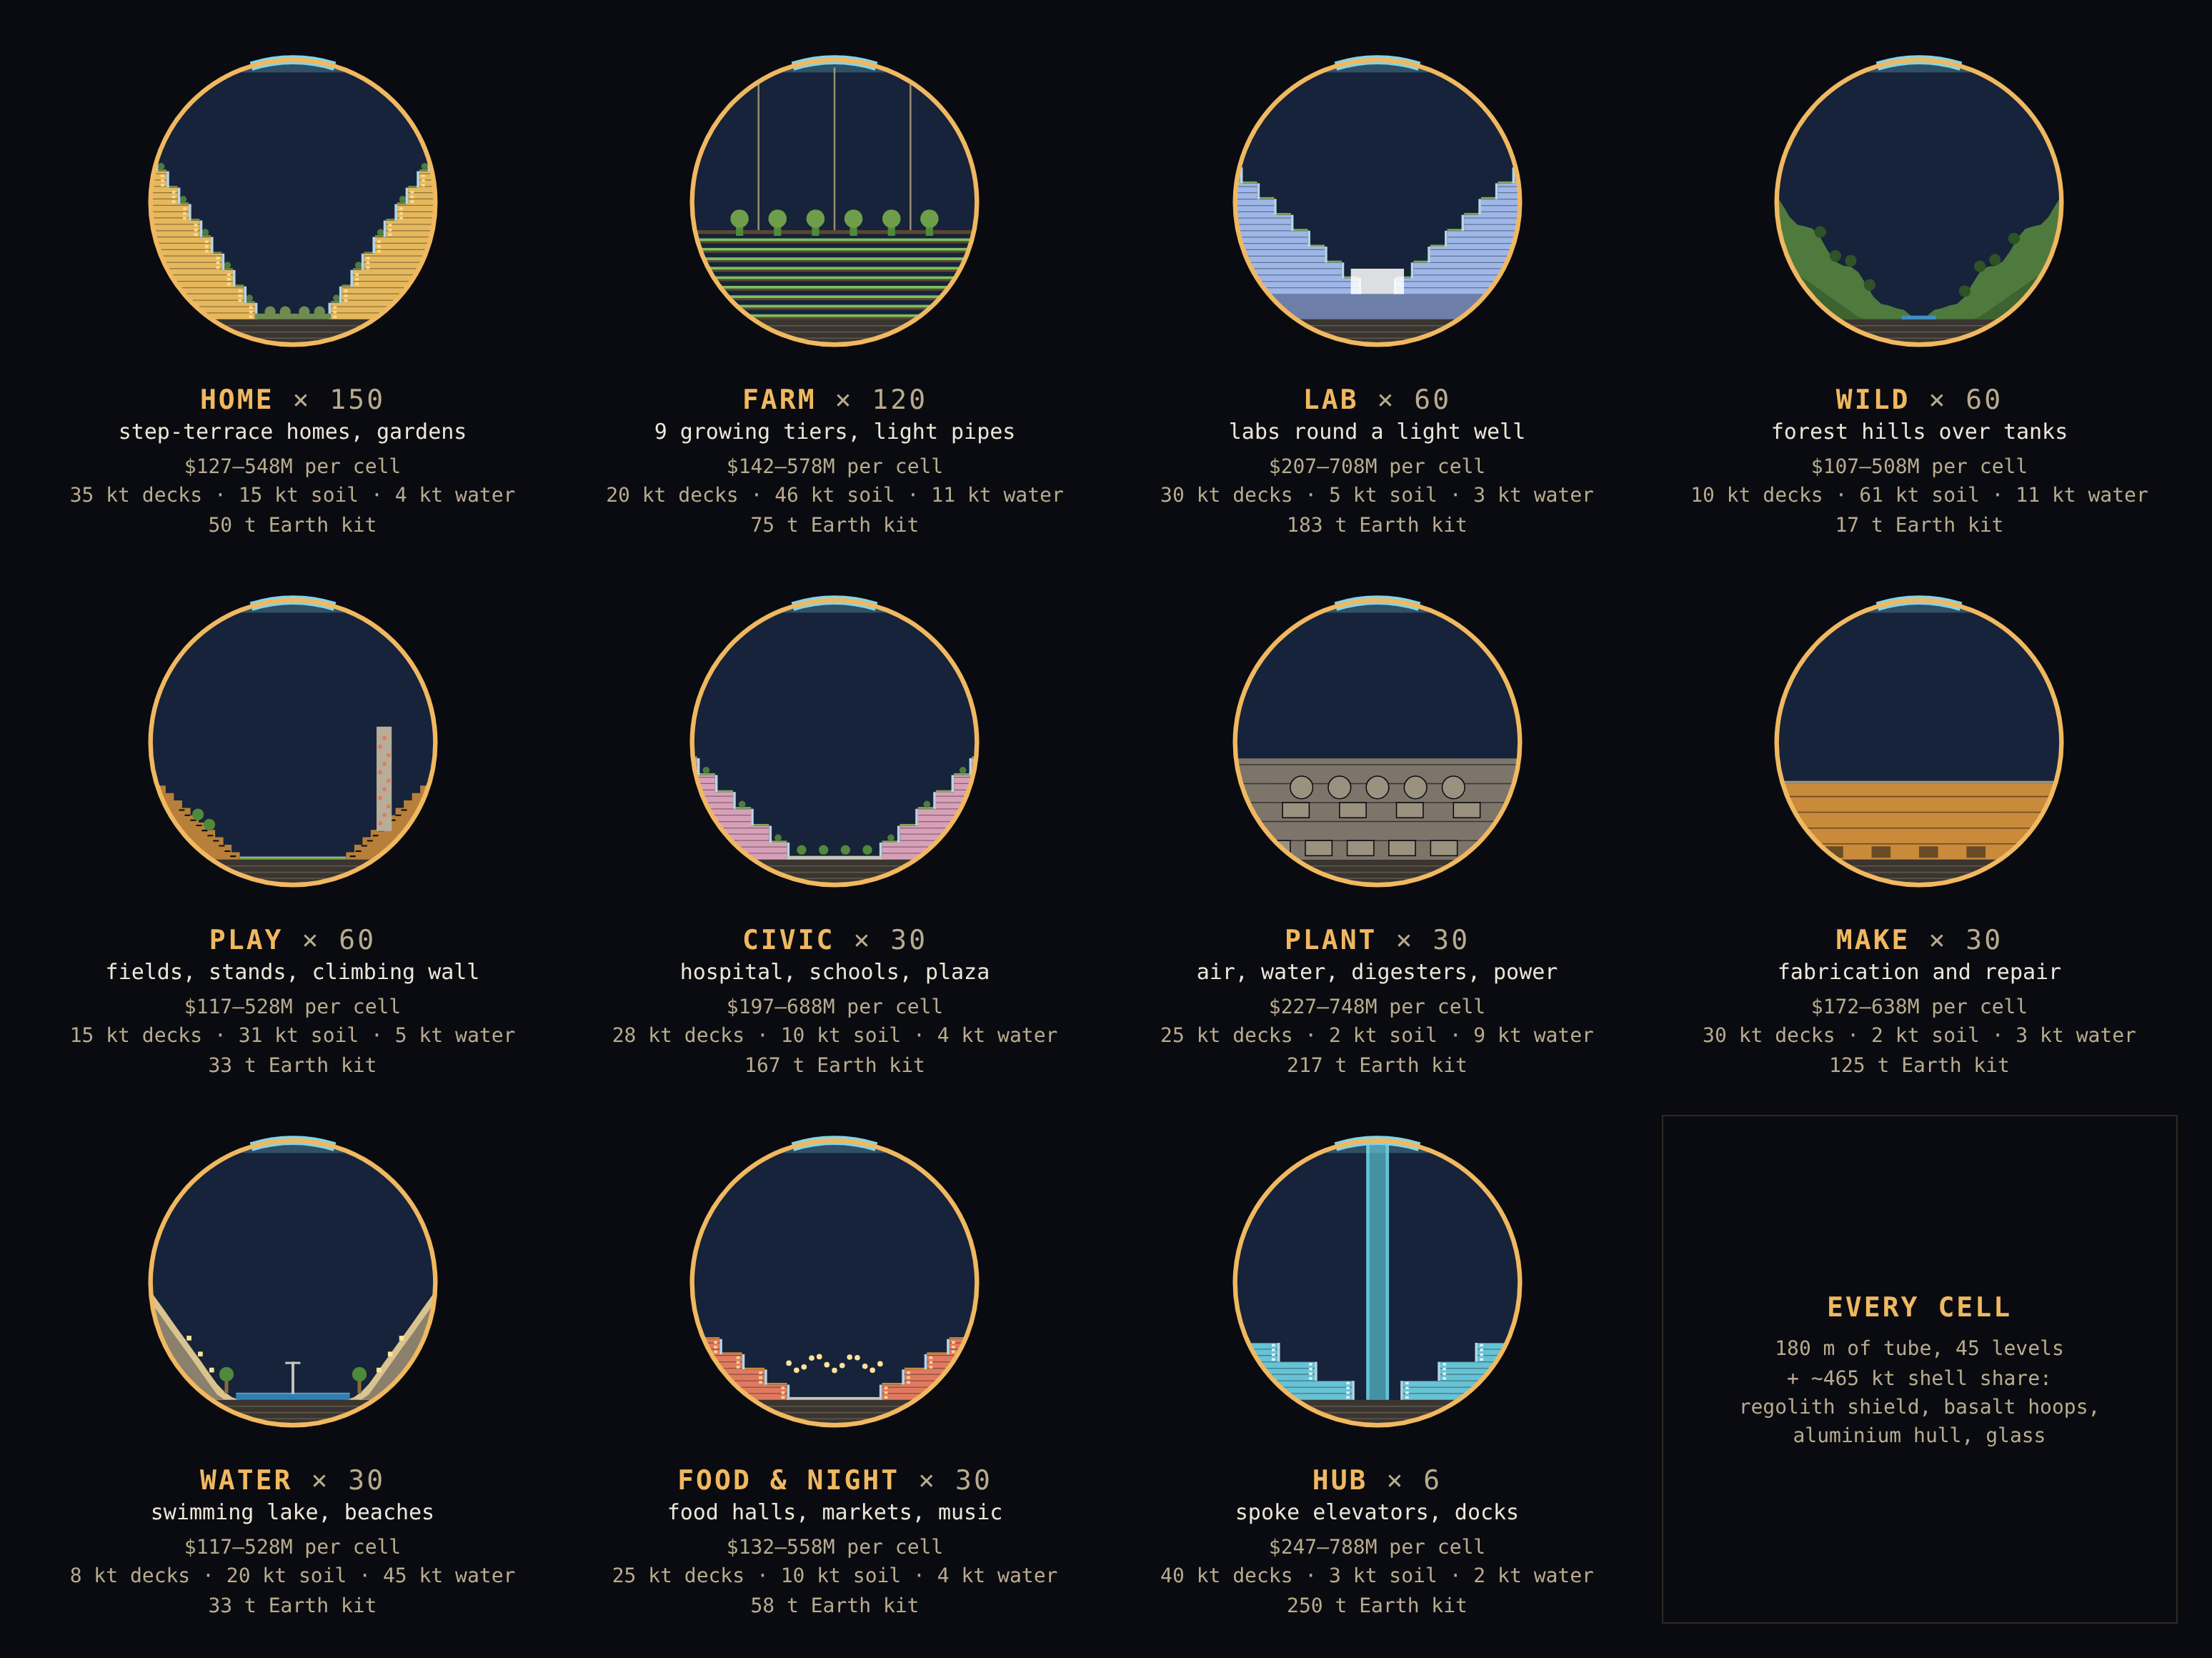
\includegraphics[width=\textwidth]{figures/cell_gallery.png}
  \caption{The 11 cell types, with their count per ring, build cost per cell, lunar interior mass and Earth kit.}
\end{figure}

\paragraph{How the cost is split.} The ring's standalone cost (\$89B optimistic, \$356B conservative) is the sum of six items from the cost model: share of the lunar industry, Earth high-tech kit, nitrogen, the power system, robots and bay factories, and design and start-up. Five of these are shared equally by all cells (\$97M a cell optimistic, \$488M conservative). The Earth kit is split by what each type needs: a hub cell carries 250\,t of elevators, docks and controls, a wild cell only 17\,t of pumps and sensors.

\begin{table}[H]
  \centering\small
  \begin{tabularx}{\textwidth}{@{}lrrrrrrX@{}}
\toprule
\textbf{Cell type} & \textbf{Cells} & \textbf{Decks} & \textbf{Soil} & \textbf{Water} & \textbf{Earth kit} & \textbf{Cost per cell} & \textbf{All cells of this type}\\
 & & kt & kt & kt & t & \$M & \$B\\
\midrule
Home & 150 & 35 & 15 & 4 & 50 & 127--548 & 19.1--82.3\\
Farm & 120 & 20 & 46 & 11 & 75 & 142--578 & 17.1--69.4\\
Lab & 60 & 30 & 5 & 3 & 183 & 207--708 & 12.4--42.5\\
Wild & 60 & 10 & 61 & 11 & 17 & 107--508 & 6.4--30.5\\
Play & 60 & 15 & 31 & 5 & 33 & 117--528 & 7.0--31.7\\
Civic & 30 & 28 & 10 & 4 & 167 & 197--688 & 5.9--20.7\\
Plant & 30 & 25 & 2 & 9 & 217 & 227--748 & 6.8--22.5\\
Make & 30 & 30 & 2 & 3 & 125 & 172--638 & 5.2--19.2\\
Water & 30 & 8 & 20 & 45 & 33 & 117--528 & 3.5--15.9\\
Food \& night & 30 & 25 & 10 & 4 & 58 & 132--558 & 4.0--16.8\\
Hub & 6 & 40 & 3 & 2 & 250 & 247--788 & 1.5--4.7\\
\midrule
\textbf{Ring} & 606 & 14.7 Mt & 15.0 Mt & 5.0 Mt & 50,000 & & \textbf{89--356}\\
\bottomrule
\end{tabularx}
  \caption{Lunar interior mass, Earth kit and build cost for each cell type. Shell mass is equal for all cells and not shown. Ranges are optimistic--conservative.}
\end{table}

\begin{figure}[H]
  \centering
  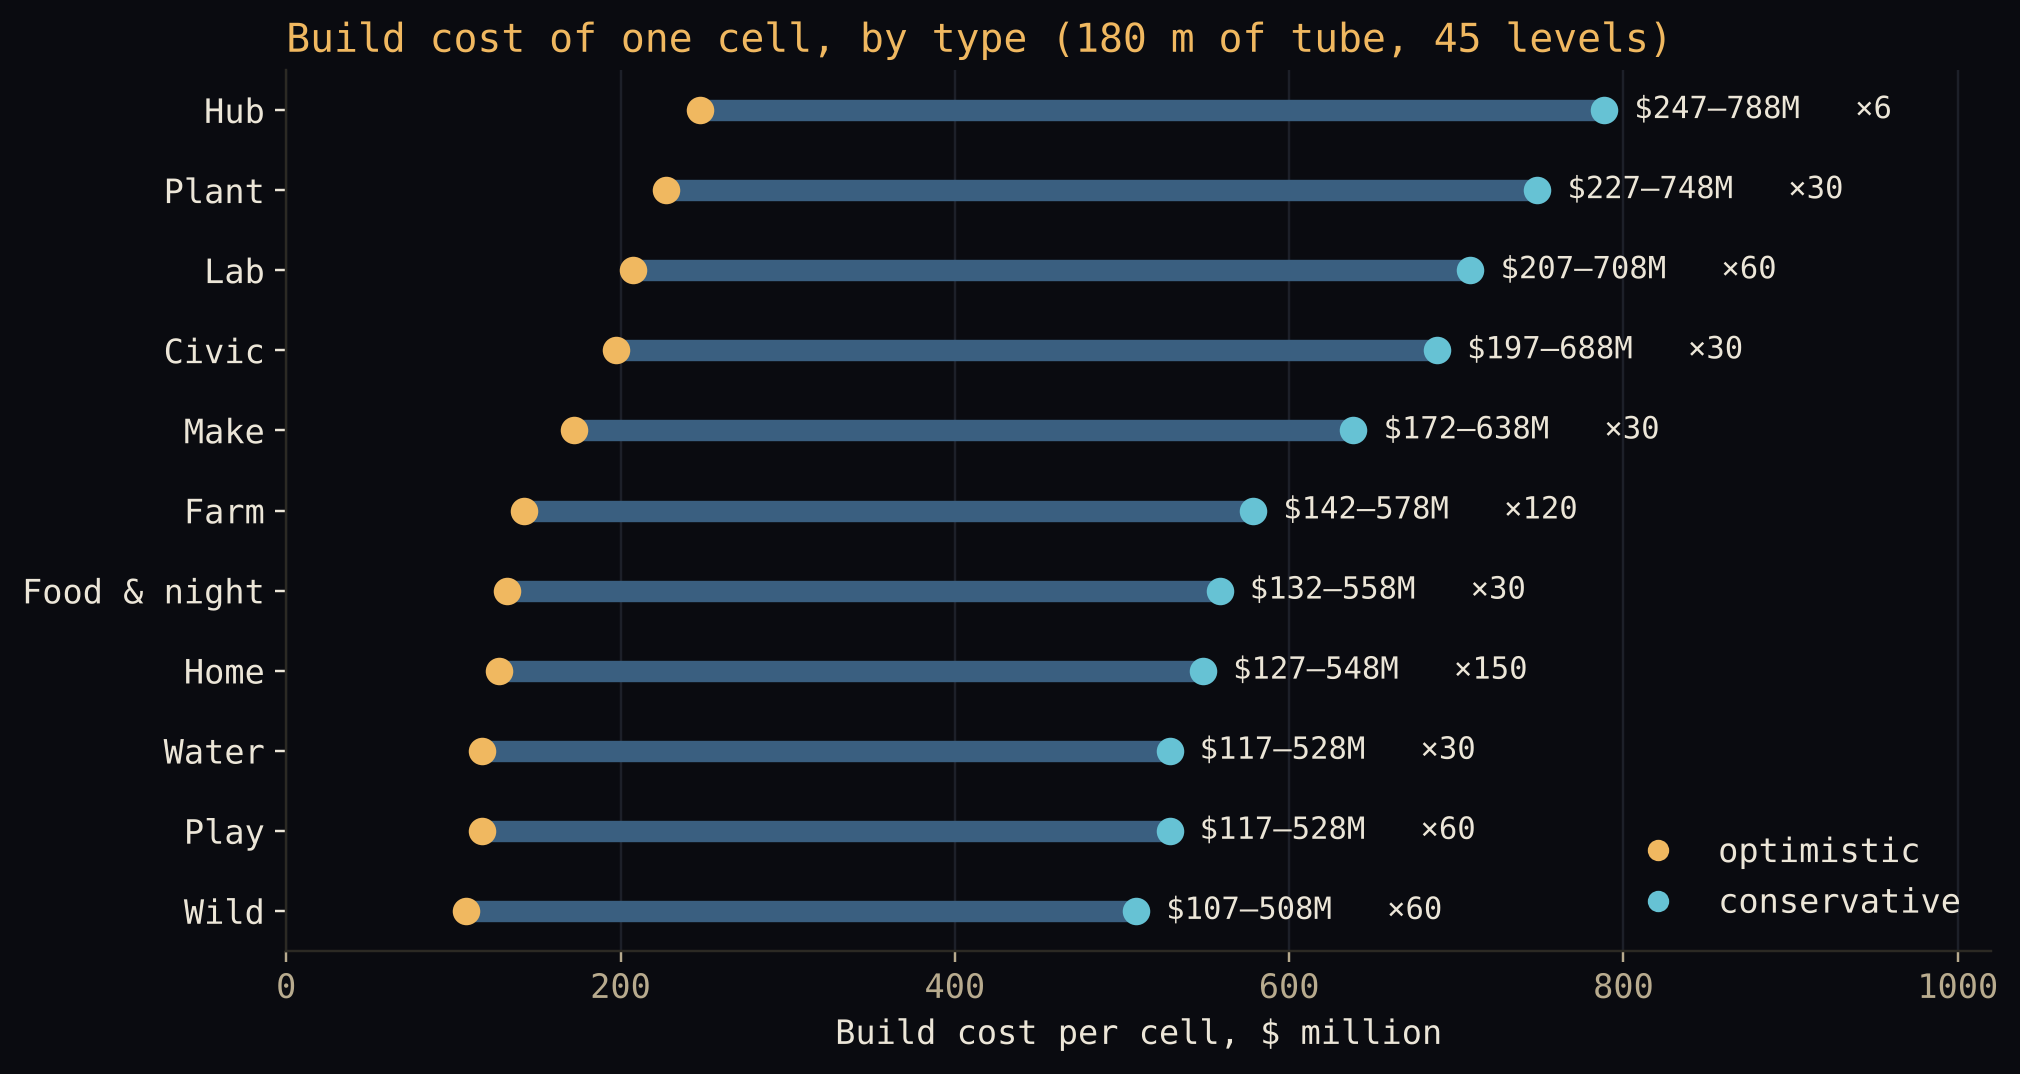
\includegraphics[width=0.9\textwidth]{figures/cost_per_cell.png}
  \caption{Build cost of one cell, by type. The spread is set mostly by nitrogen and power prices, not by the cell's own fit-out.}
\end{figure}

\begin{figure}[H]
  \centering
  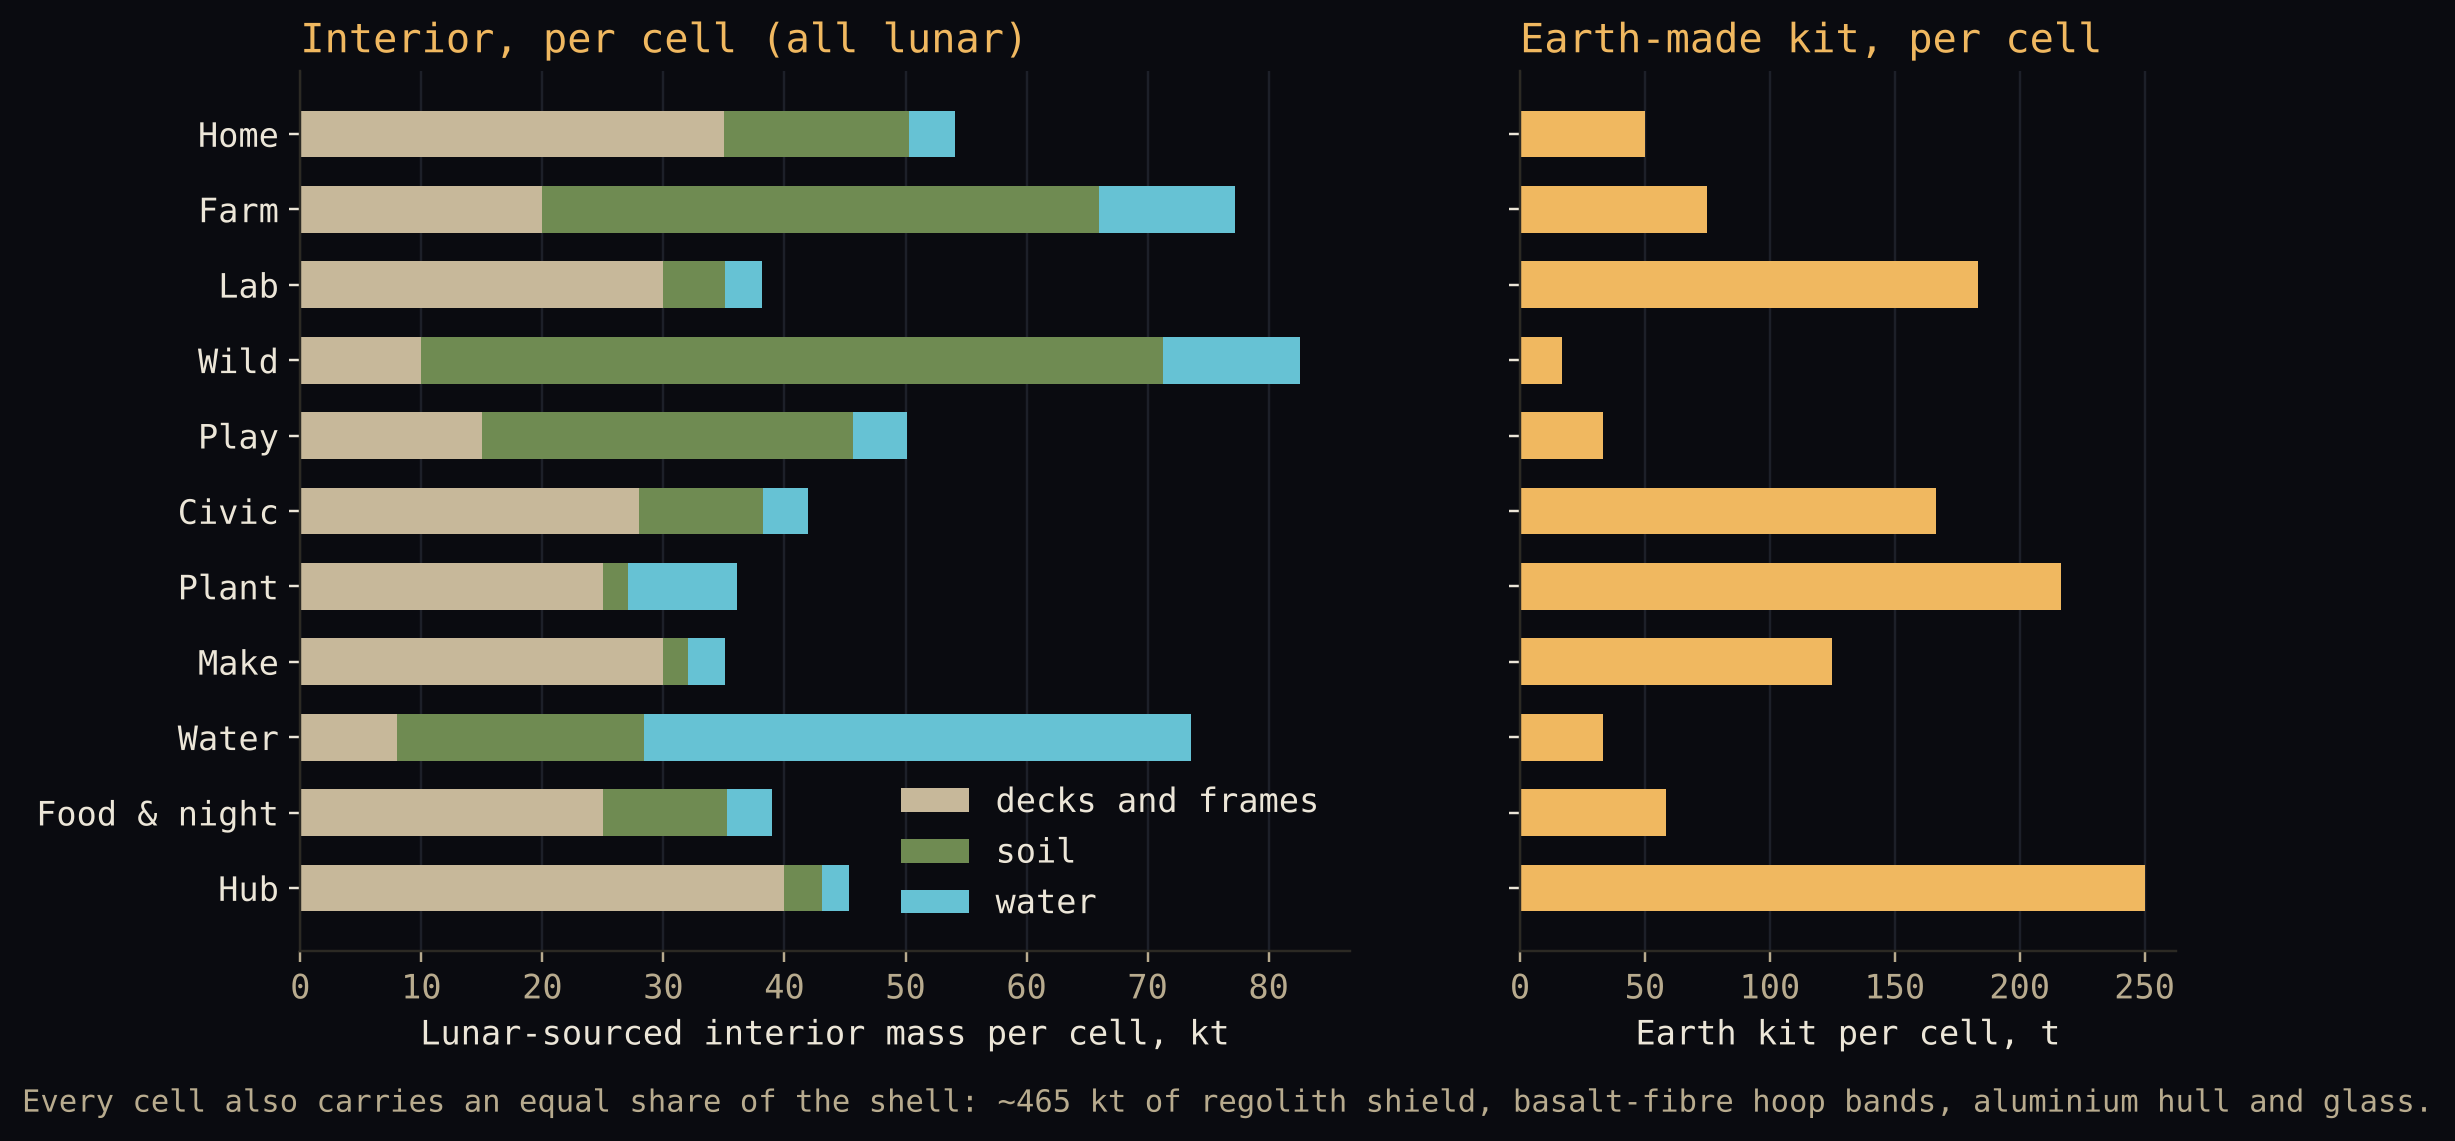
\includegraphics[width=\textwidth]{figures/mass_per_cell.png}
  \caption{What goes inside each cell type: lunar decks, soil and water (left) and Earth-made kit (right).}
\end{figure}

\begin{figure}[H]
  \centering
  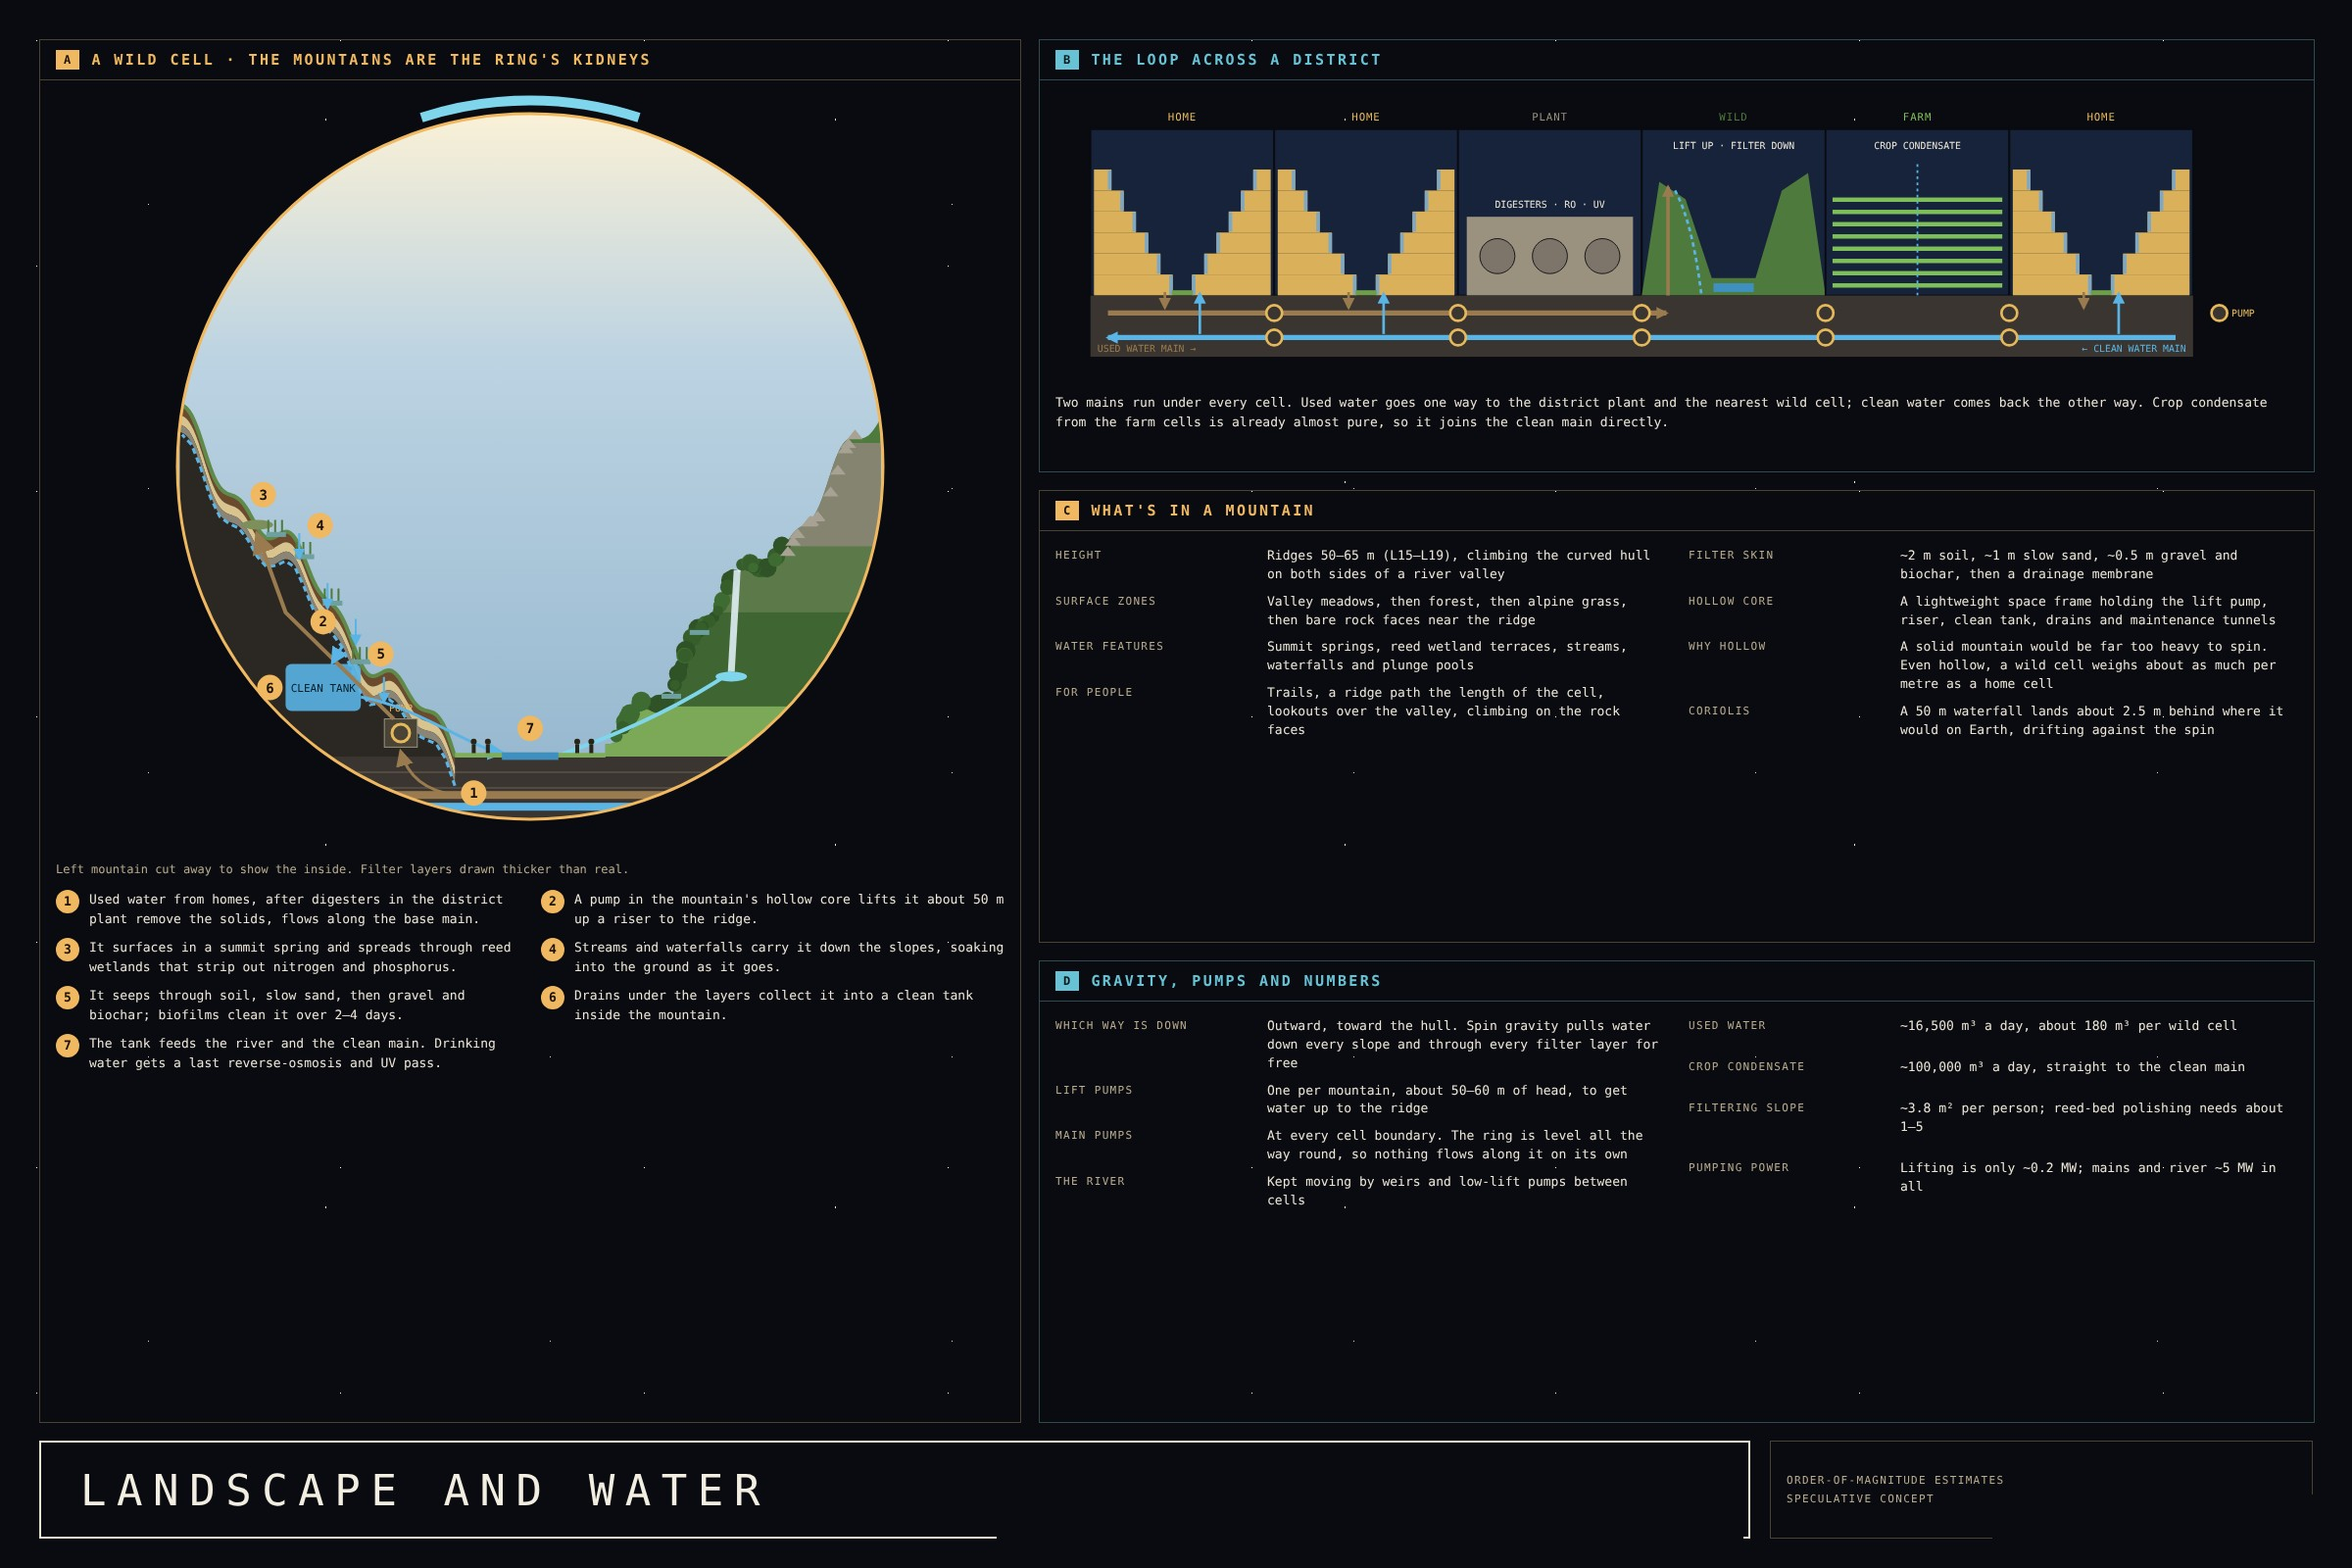
\includegraphics[width=\textwidth]{figures/board-landscape-and-water.jpg}
  \caption{Design board: hollow filter mountains and the district water loop, which set the soil and water mass of the wild, water and farm cells.}
\end{figure}

\begin{figure}[H]
  \centering
  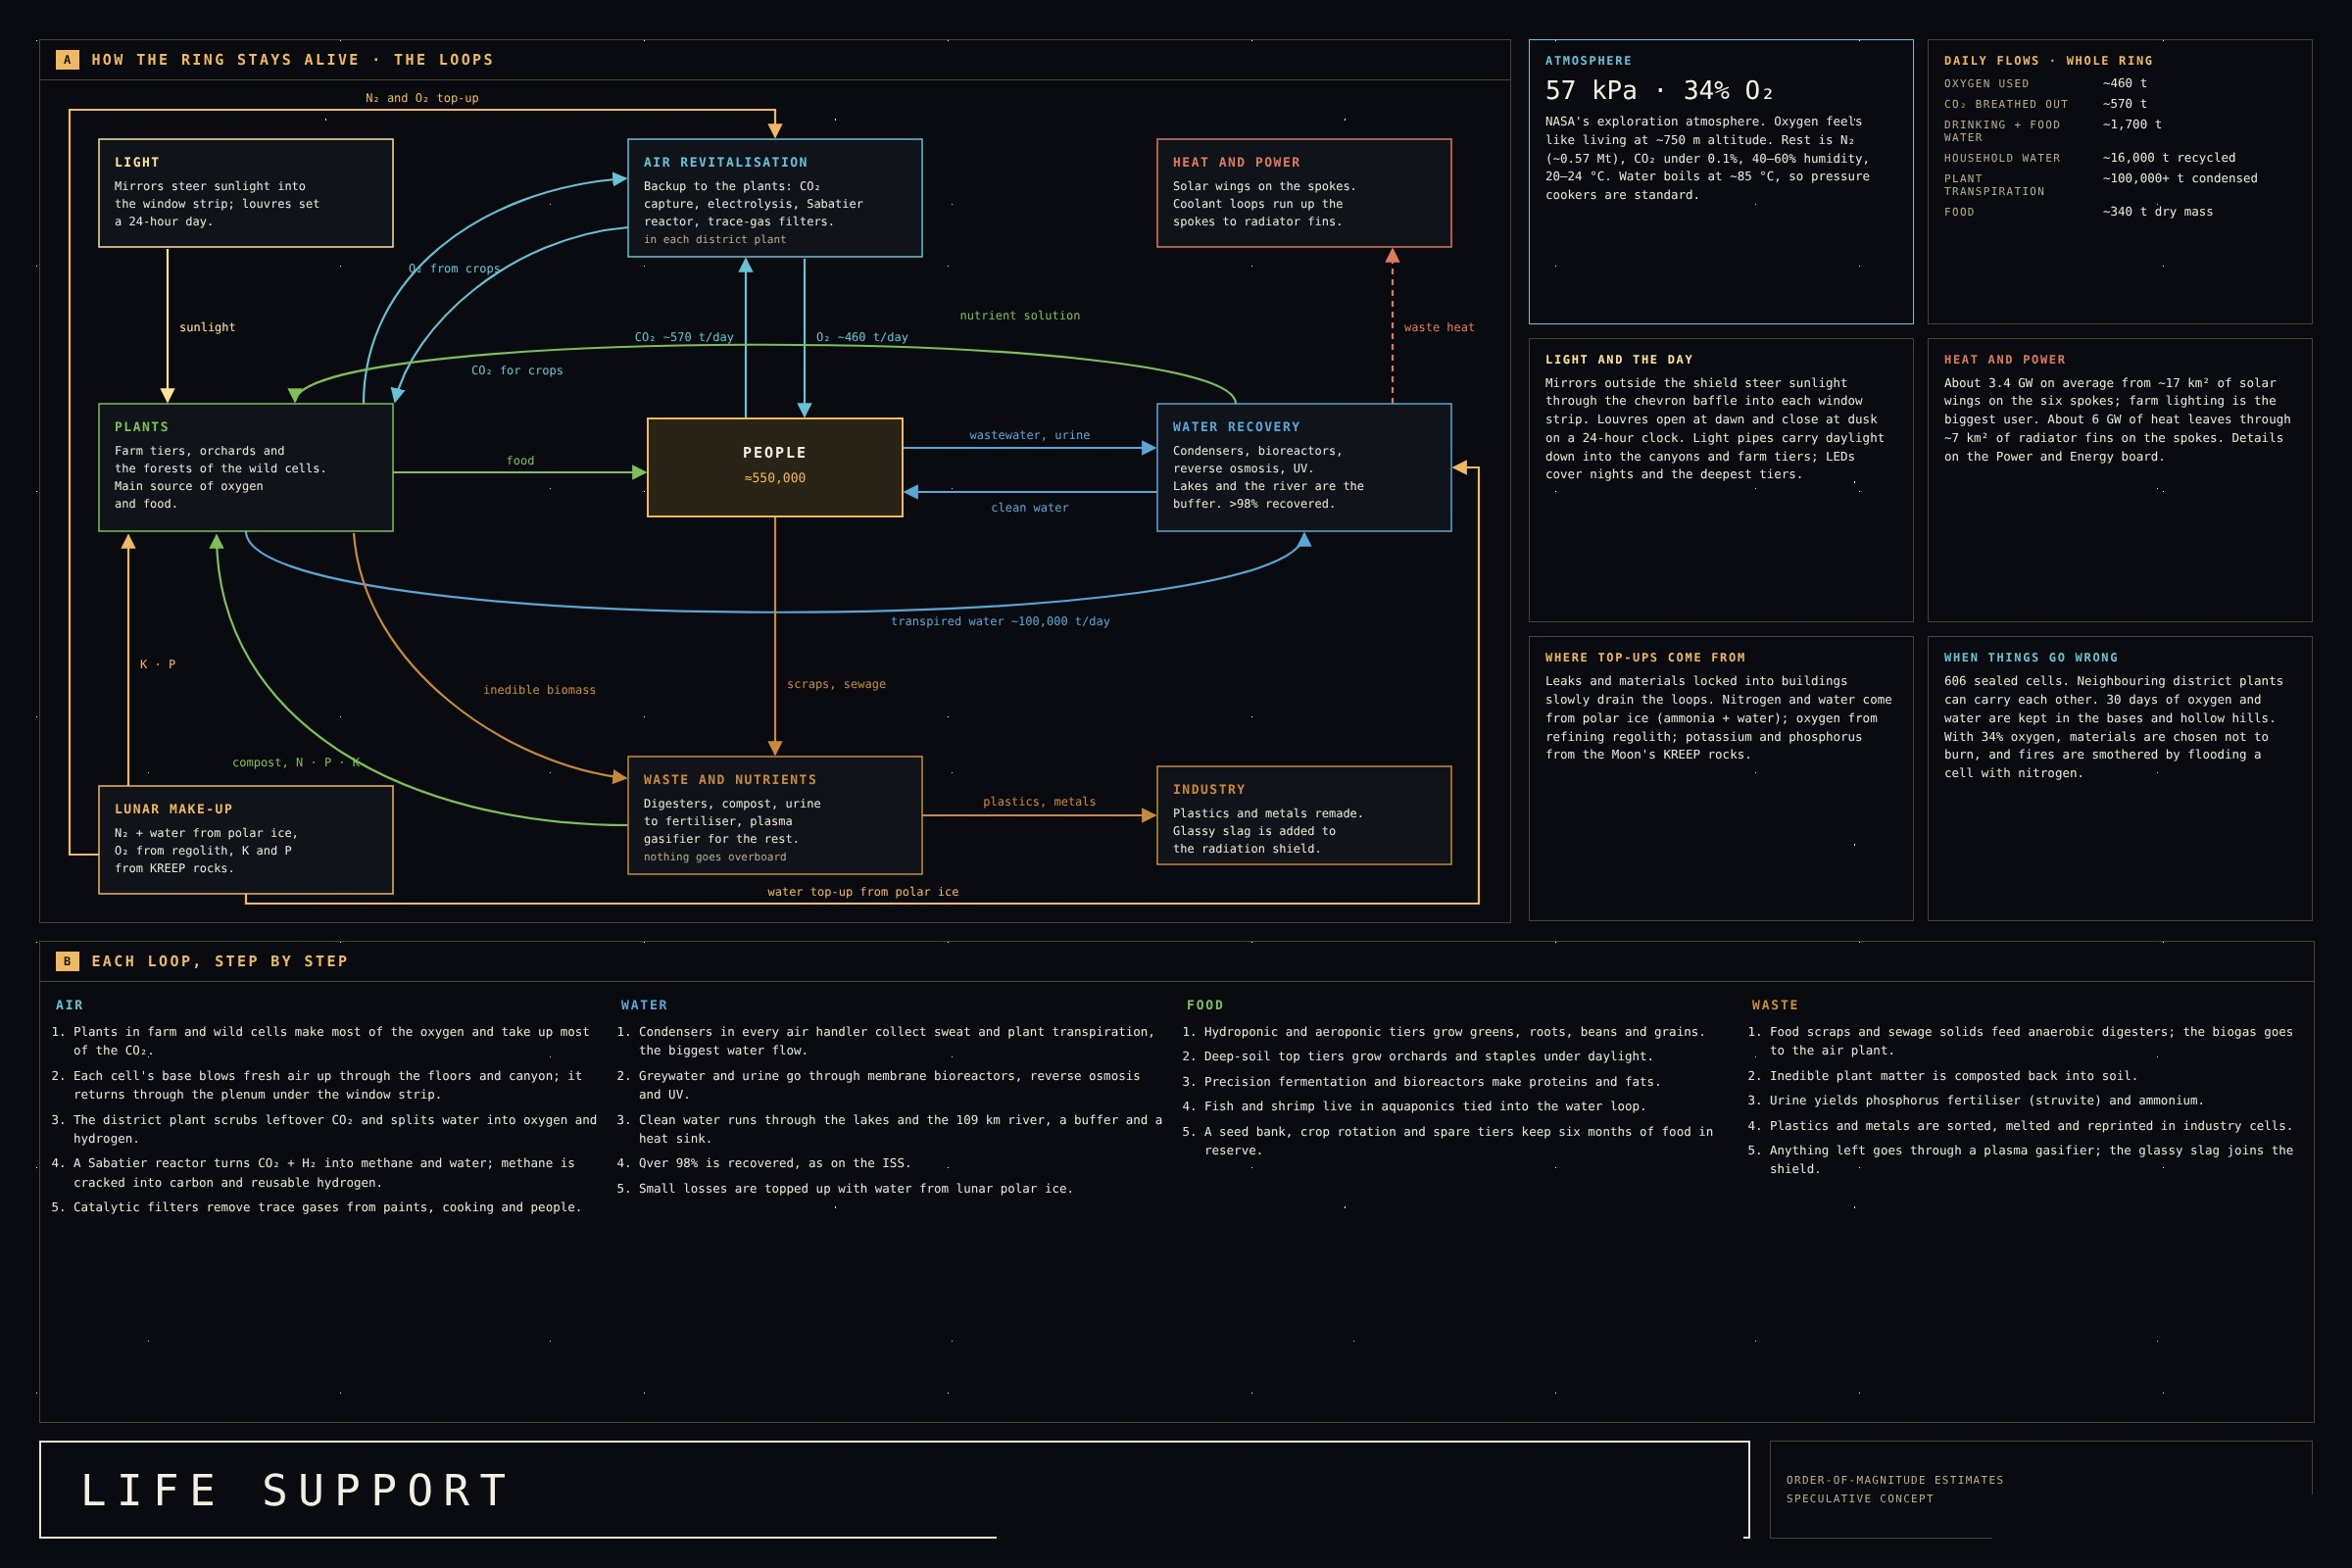
\includegraphics[width=\textwidth]{figures/board-life-support.jpg}
  \caption{Design board: air, water, food and waste loops. Most of the Earth kit in plant and farm cells is this machinery.}
\end{figure}

\section{The lunar base}
One mass-driver line delivers 30\,Mt a year, enough for one ring about every 10 years. Rings faster than that need more lines: ten lines give a ring a year. The base sits on a polar ridge with near-constant sunlight, next to a permanently shadowed crater for ice and within haul range of mare and highland regolith.

\begin{figure}[H]
  \centering
  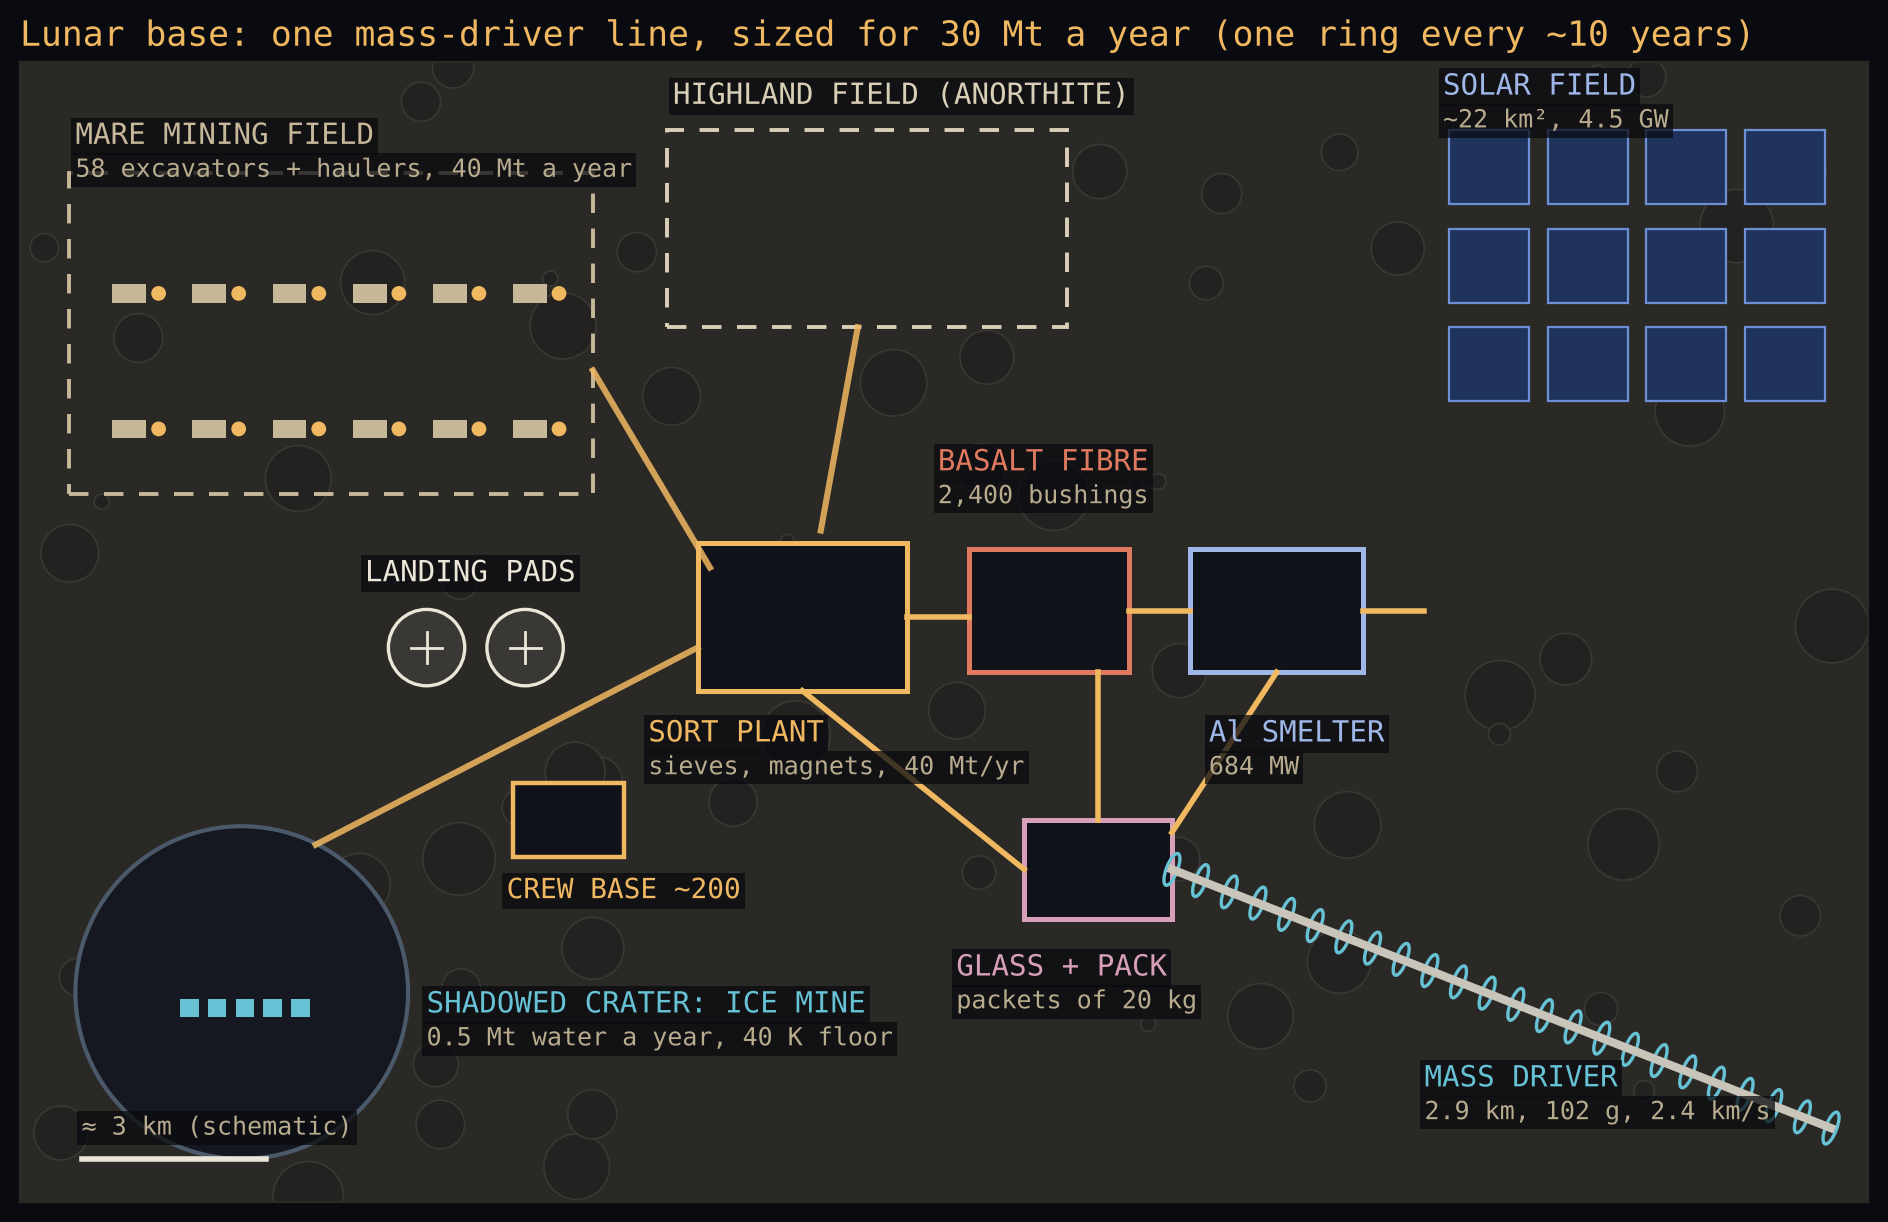
\includegraphics[width=\textwidth]{figures/lunar_site.png}
  \caption{Lunar base site plan (schematic): mining fields, sort plant, fibre works, smelter, glass and packing, ice mine, solar field, landing pads and the mass driver.}
\end{figure}

\begin{table}[H]
  \centering\small
  \begin{tabularx}{\textwidth}{@{}lXr@{}}
\toprule
\textbf{Unit} & \textbf{Spec} & \textbf{Power}\\
\midrule
Mining fleet & 58 bucket-wheel excavators (100 t/h each, 7,000 h/yr) plus haulers; 40 Mt/yr of regolith dug from mare and highland fields & \multirow{2}{*}{91 MW}\\
Sort plant & Sieves, magnetic and electrostatic separation; about 75\% of the feed is shipped, the rest is tailings & \\
Basalt fibre works & Electric furnaces at 1,500\,\textdegree C feeding 2,400 platinum--rhodium bushings (100 kg/h each); 1.8 Mt/yr of continuous fibre & 57 MW\\
Aluminium smelter & Molten-salt electrolysis of anorthite at $\sim$15 MWh/t; 0.4 Mt/yr of aluminium and oxygen as a by-product & 684 MW\\
Glass line & Regolith melt to window glass; 0.1 Mt/yr & 6 MW\\
Ice mine & Rovers and heated tents in a permanently shadowed crater (40 K floor); 0.5 Mt/yr of water & 57 MW\\
Packer and mass driver & 20 kg packets, 48 a second; 2.88 km coilgun at 102\,g to 2.4 km/s; 30 Mt/yr & 3,422 MW\\
Crew base, pads, workshops & $\sim$200 crew, 2 landing pads of sintered regolith, robot repair shops & 150 MW\\
\midrule
\textbf{Solar field} & $\sim$22 km\textsuperscript{2} of arrays at $\sim$200 W/m\textsuperscript{2} on a polar ridge with near-constant sun & \textbf{4.5 GW}\\
\bottomrule
\end{tabularx}
  \caption{Lunar base units for one mass-driver line, with their electrical demand.}
\end{table}

\begin{figure}[H]
  \centering
  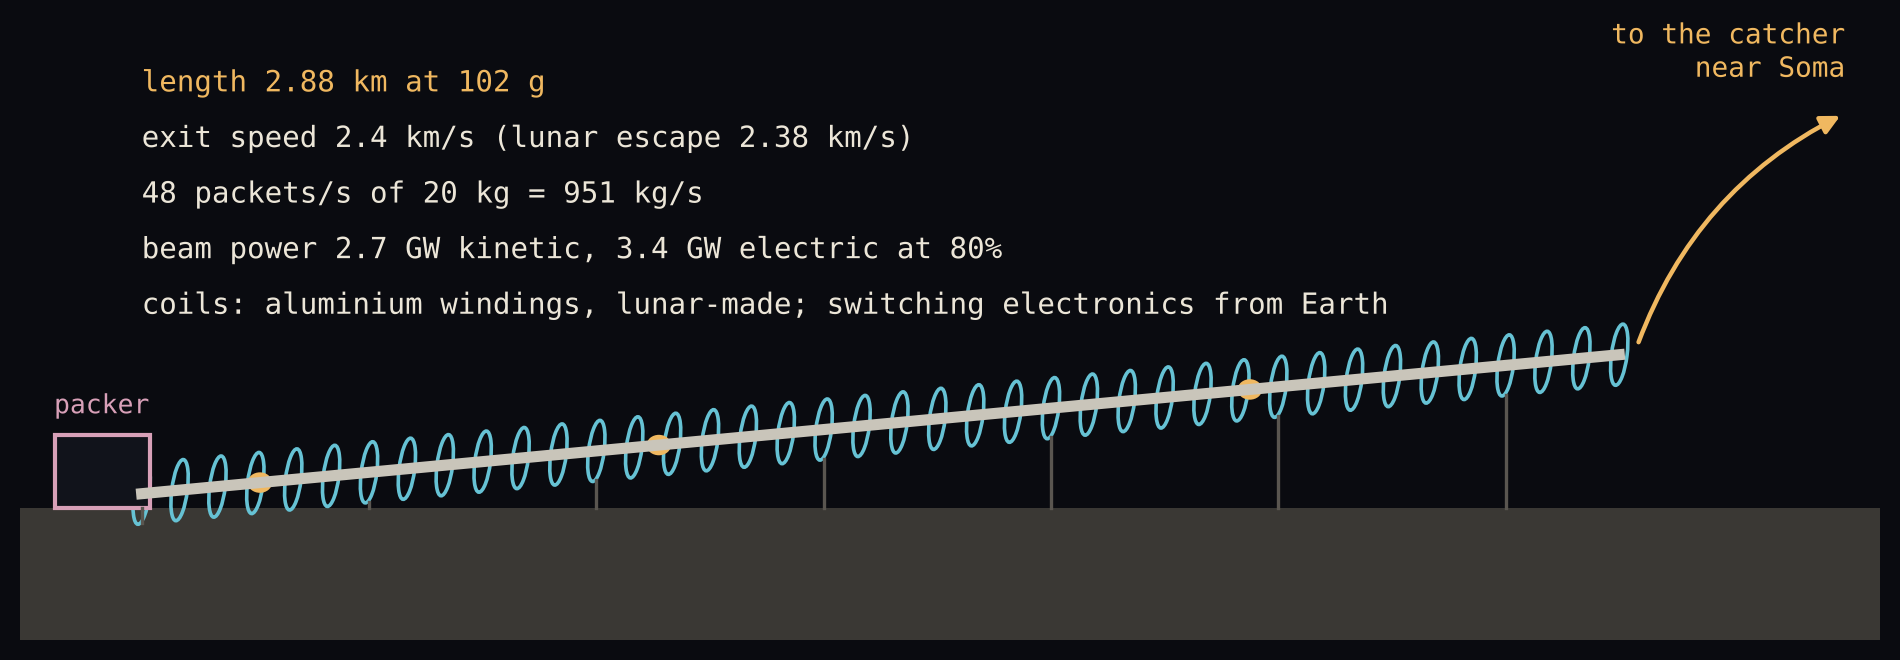
\includegraphics[width=\textwidth]{figures/mass_driver.png}
  \caption{The mass driver: a coilgun that throws 20\,kg packets just above lunar escape speed toward a catcher near Soma.}
\end{figure}

The launch speed sets the length and the power:
\begin{equation}
  L = \frac{v^2}{2a} = \frac{(2400\ \mathrm{m\,s^{-1}})^2}{2 \times 1000\ \mathrm{m\,s^{-2}}} \approx 2.9\ \mathrm{km}, \qquad
  P = \tfrac{1}{2}\,\dot m\,v^2 = \tfrac{1}{2} \times 951\ \mathrm{kg\,s^{-1}} \times (2400\ \mathrm{m\,s^{-1}})^2 \approx 2.7\ \mathrm{GW}.
\end{equation}

\paragraph{Building the base.} Earth lands a 20,000\,t seed factory: excavators, a pilot sort plant, a first furnace and bushings, a small smelter, 200\,MW of arrays and a crew base. The base then grows mostly from its own output, with $\sim$250,000\,t of Earth-made parts over its life (motors, power electronics, bushings, sensors). The programme costs \$0.5--1.9T, shared by 100 rings (\$5--19B a ring).

\section{Starship launches}
Each delivery beyond low Earth orbit needs tanker flights to refuel the ship first: about 6 per 100\,t delivered to Soma's orbit and 10--15 per 100\,t landed on the Moon.

\begin{table}[H]
  \centering\small
  \begin{tabularx}{\textwidth}{@{}Xrr@{}}
\toprule
\textbf{Stage} & \textbf{Payload} & \textbf{Launches}\\
\midrule
\multicolumn{3}{@{}l}{\emph{Once, shared by all rings (to the lunar surface: 100 t a landing, 10--15 tankers each)}}\\
Lunar seed factory & 20,000 t & 2,200--3,200\\
Lunar full build-out (Earth-made parts) & 250,000 t & 27,500--40,000\\
\midrule
\multicolumn{3}{@{}l}{\emph{Each ring (to Soma's orbit: 100 t a delivery, $\sim$6 tankers each)}}\\
Spine share (280 Starships per 6-ring stack) & 47 ships & 327\\
Bay factories (6 $\times$ 7 flights) & 42 loads & 294\\
Robot fleet & 5,000 t & 350\\
Earth high-tech kit & 50,000 t & 3,500\\
Batteries & 37,500 t & 2,625\\
\textbf{Subtotal, without nitrogen} & & \textbf{7,096}\\
Nitrogen from Earth & 0.3--0.6 Mt & 21,000--42,000\\
\textbf{Per ring, all in} & & \textbf{28,096--49,096}\\
\bottomrule
\end{tabularx}
  \caption{Starship launches by stage, tanker flights included.}
\end{table}

\begin{figure}[H]
  \centering
  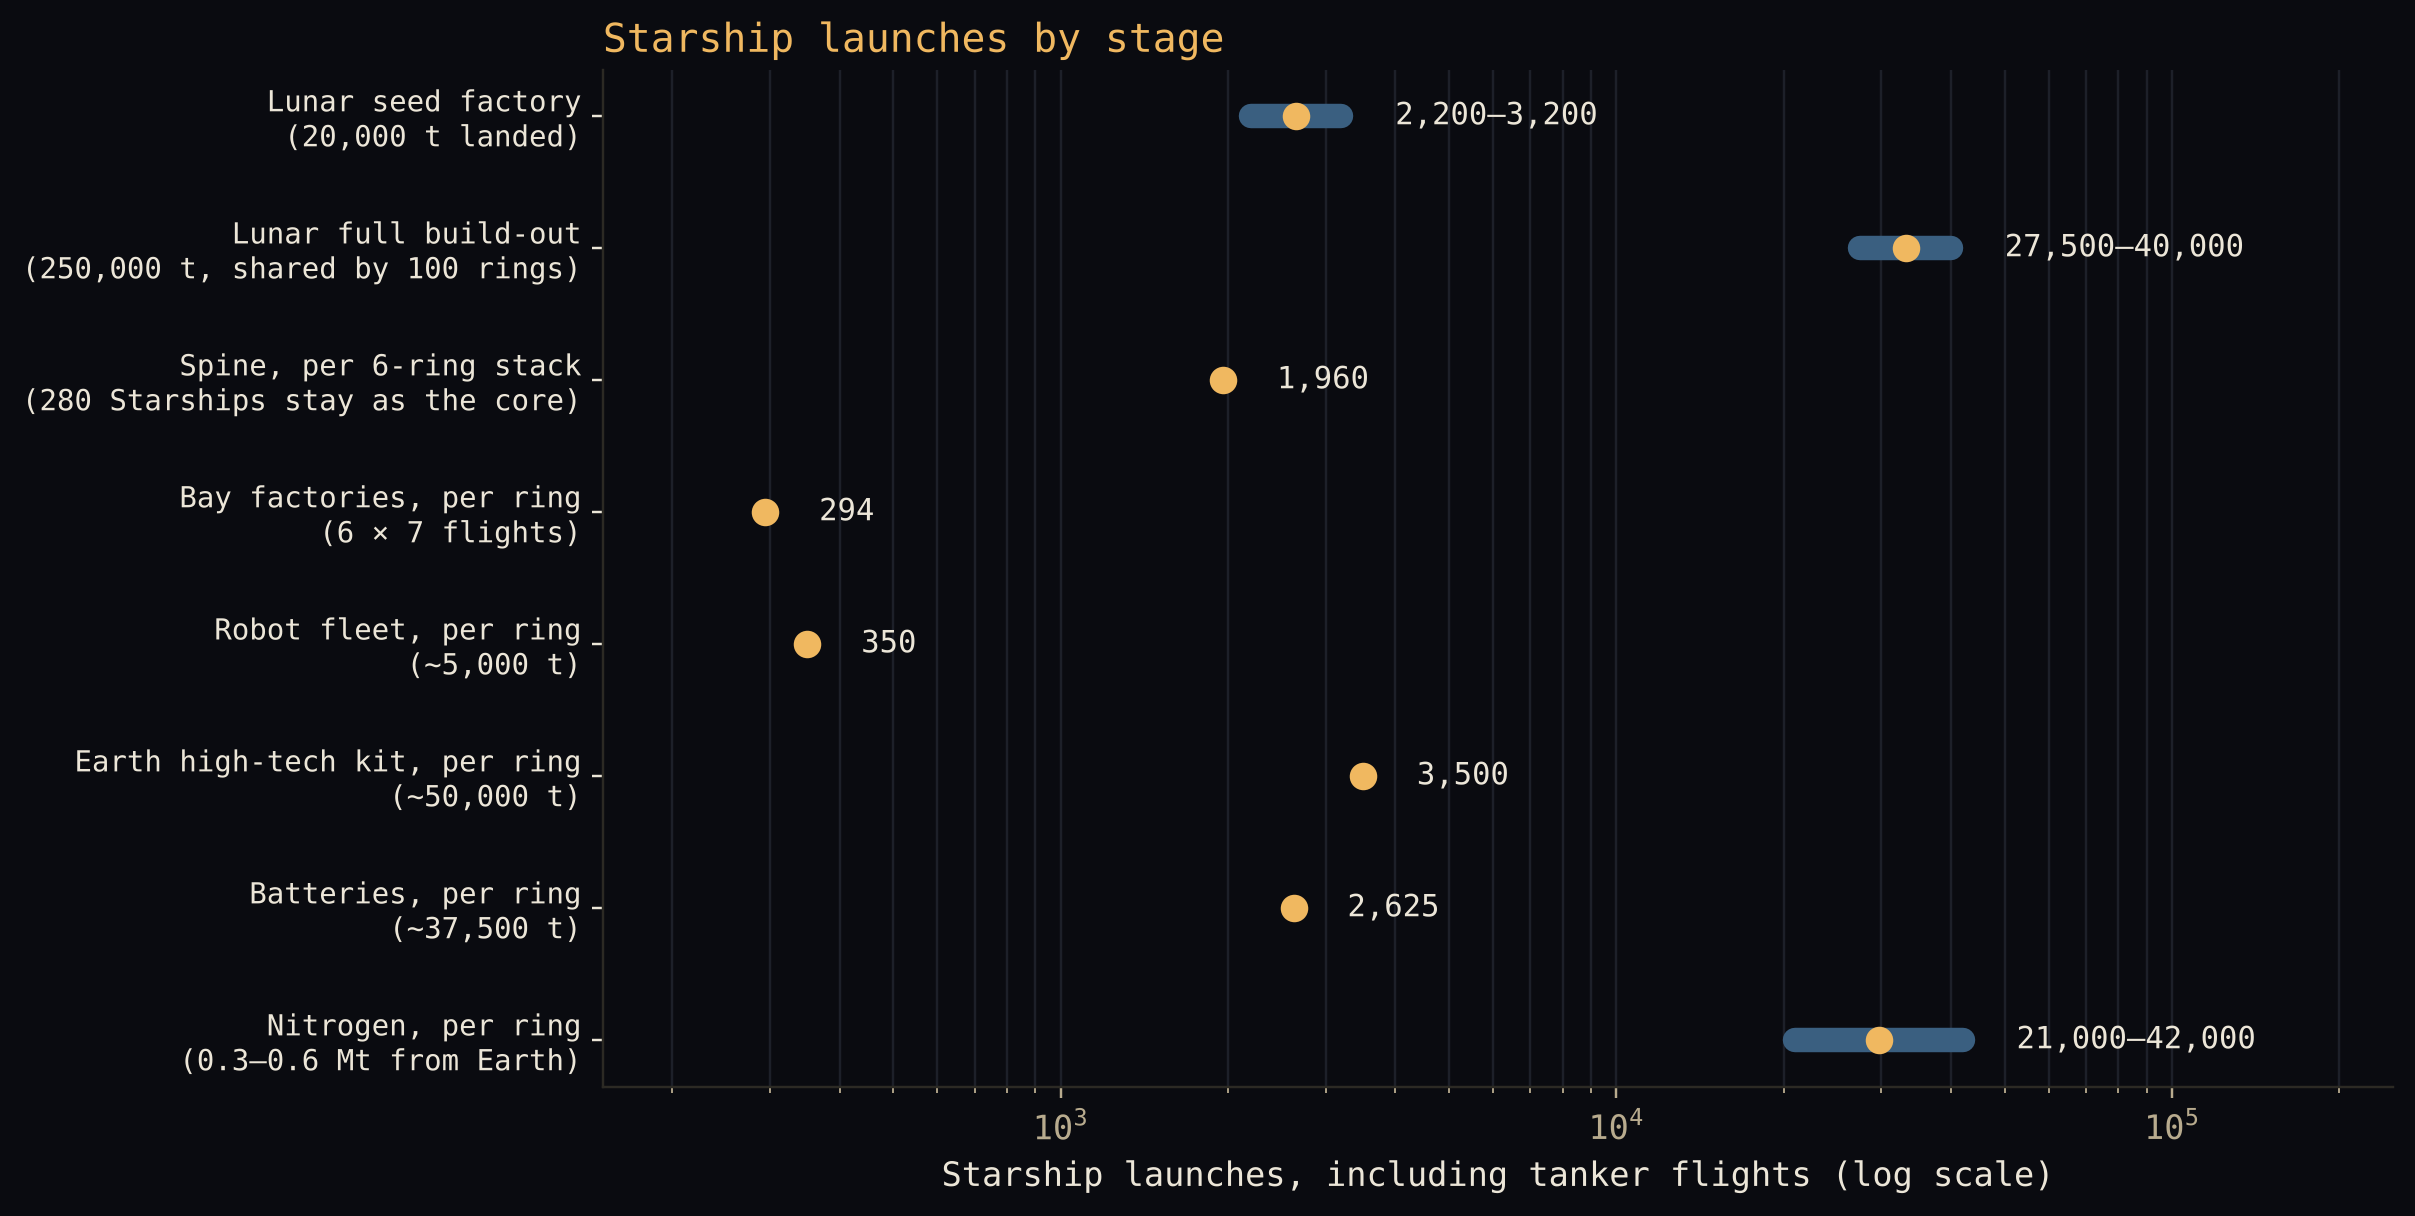
\includegraphics[width=\textwidth]{figures/launches.png}
  \caption{Launches by stage on a log scale. Nitrogen dominates: sourcing it from asteroids or lunar polar volatiles cuts a ring's launches from $\sim$28,000--49,000 to $\sim$7,100.}
\end{figure}

\begin{figure}[H]
  \centering
  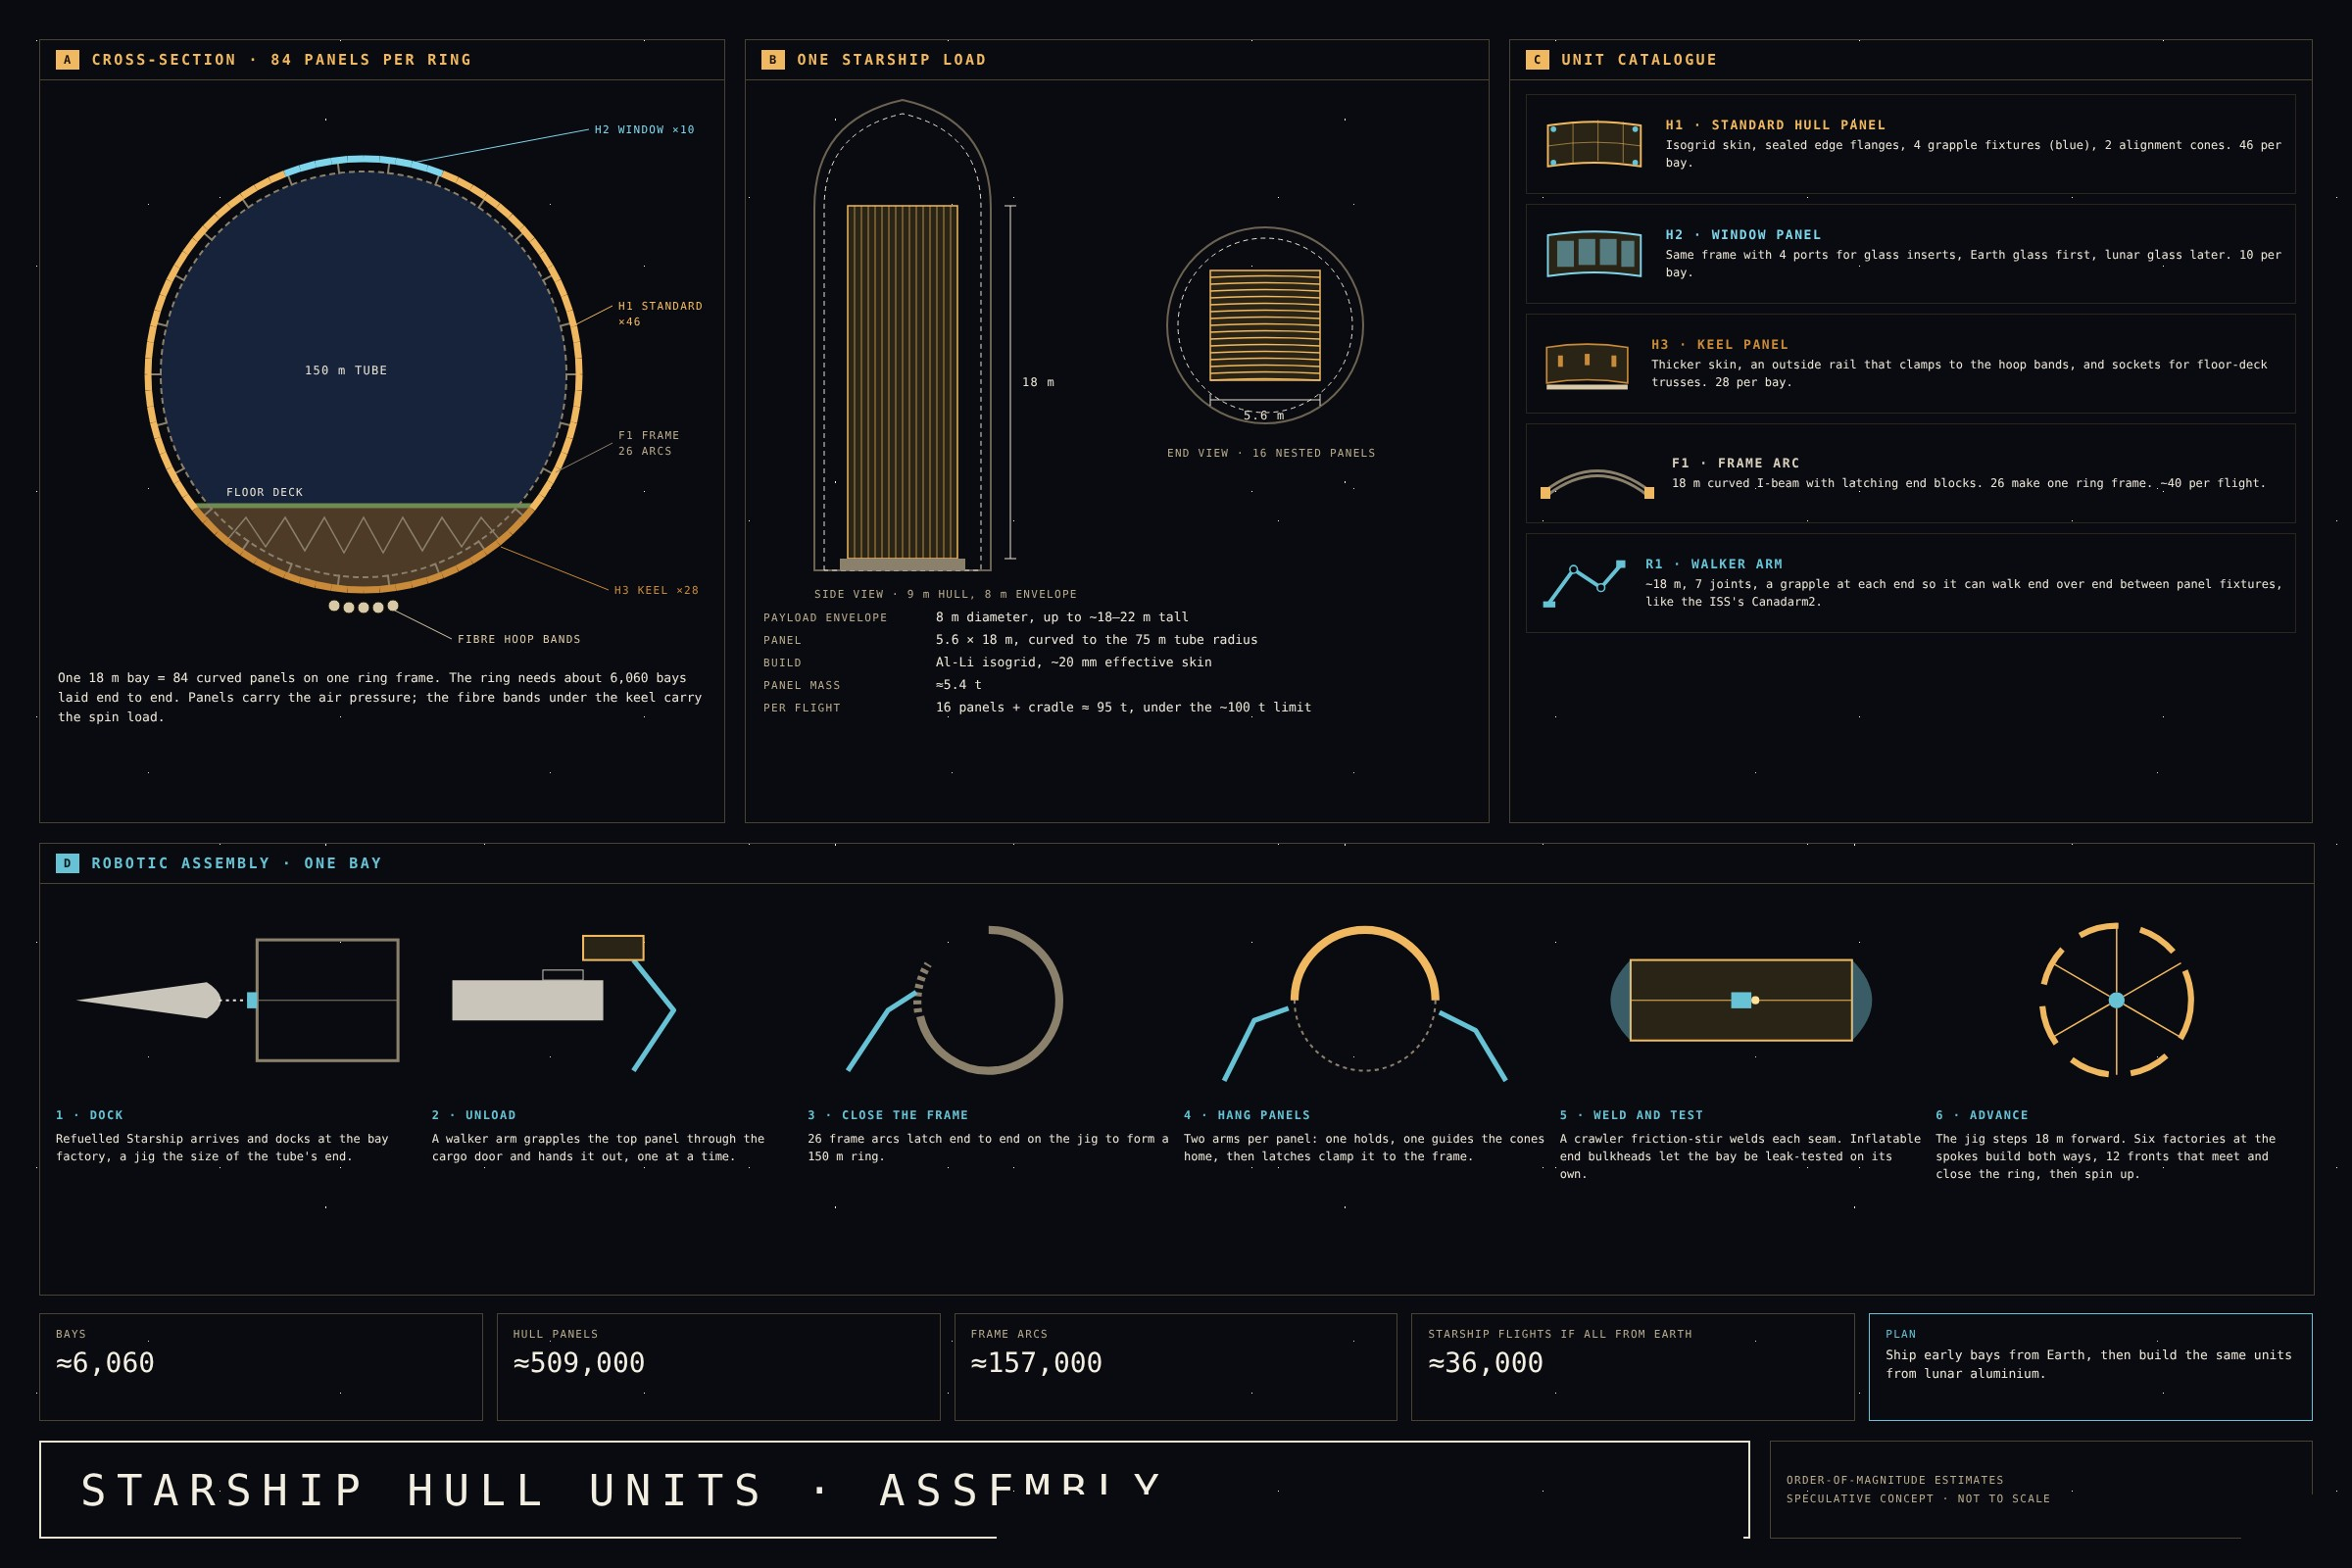
\includegraphics[width=\textwidth]{figures/board-starship-hull-units.jpg}
  \caption{Design board: Starship-sized hull units, 84 panels per bay, and robotic assembly of one bay.}
\end{figure}

\begin{figure}[H]
  \centering
  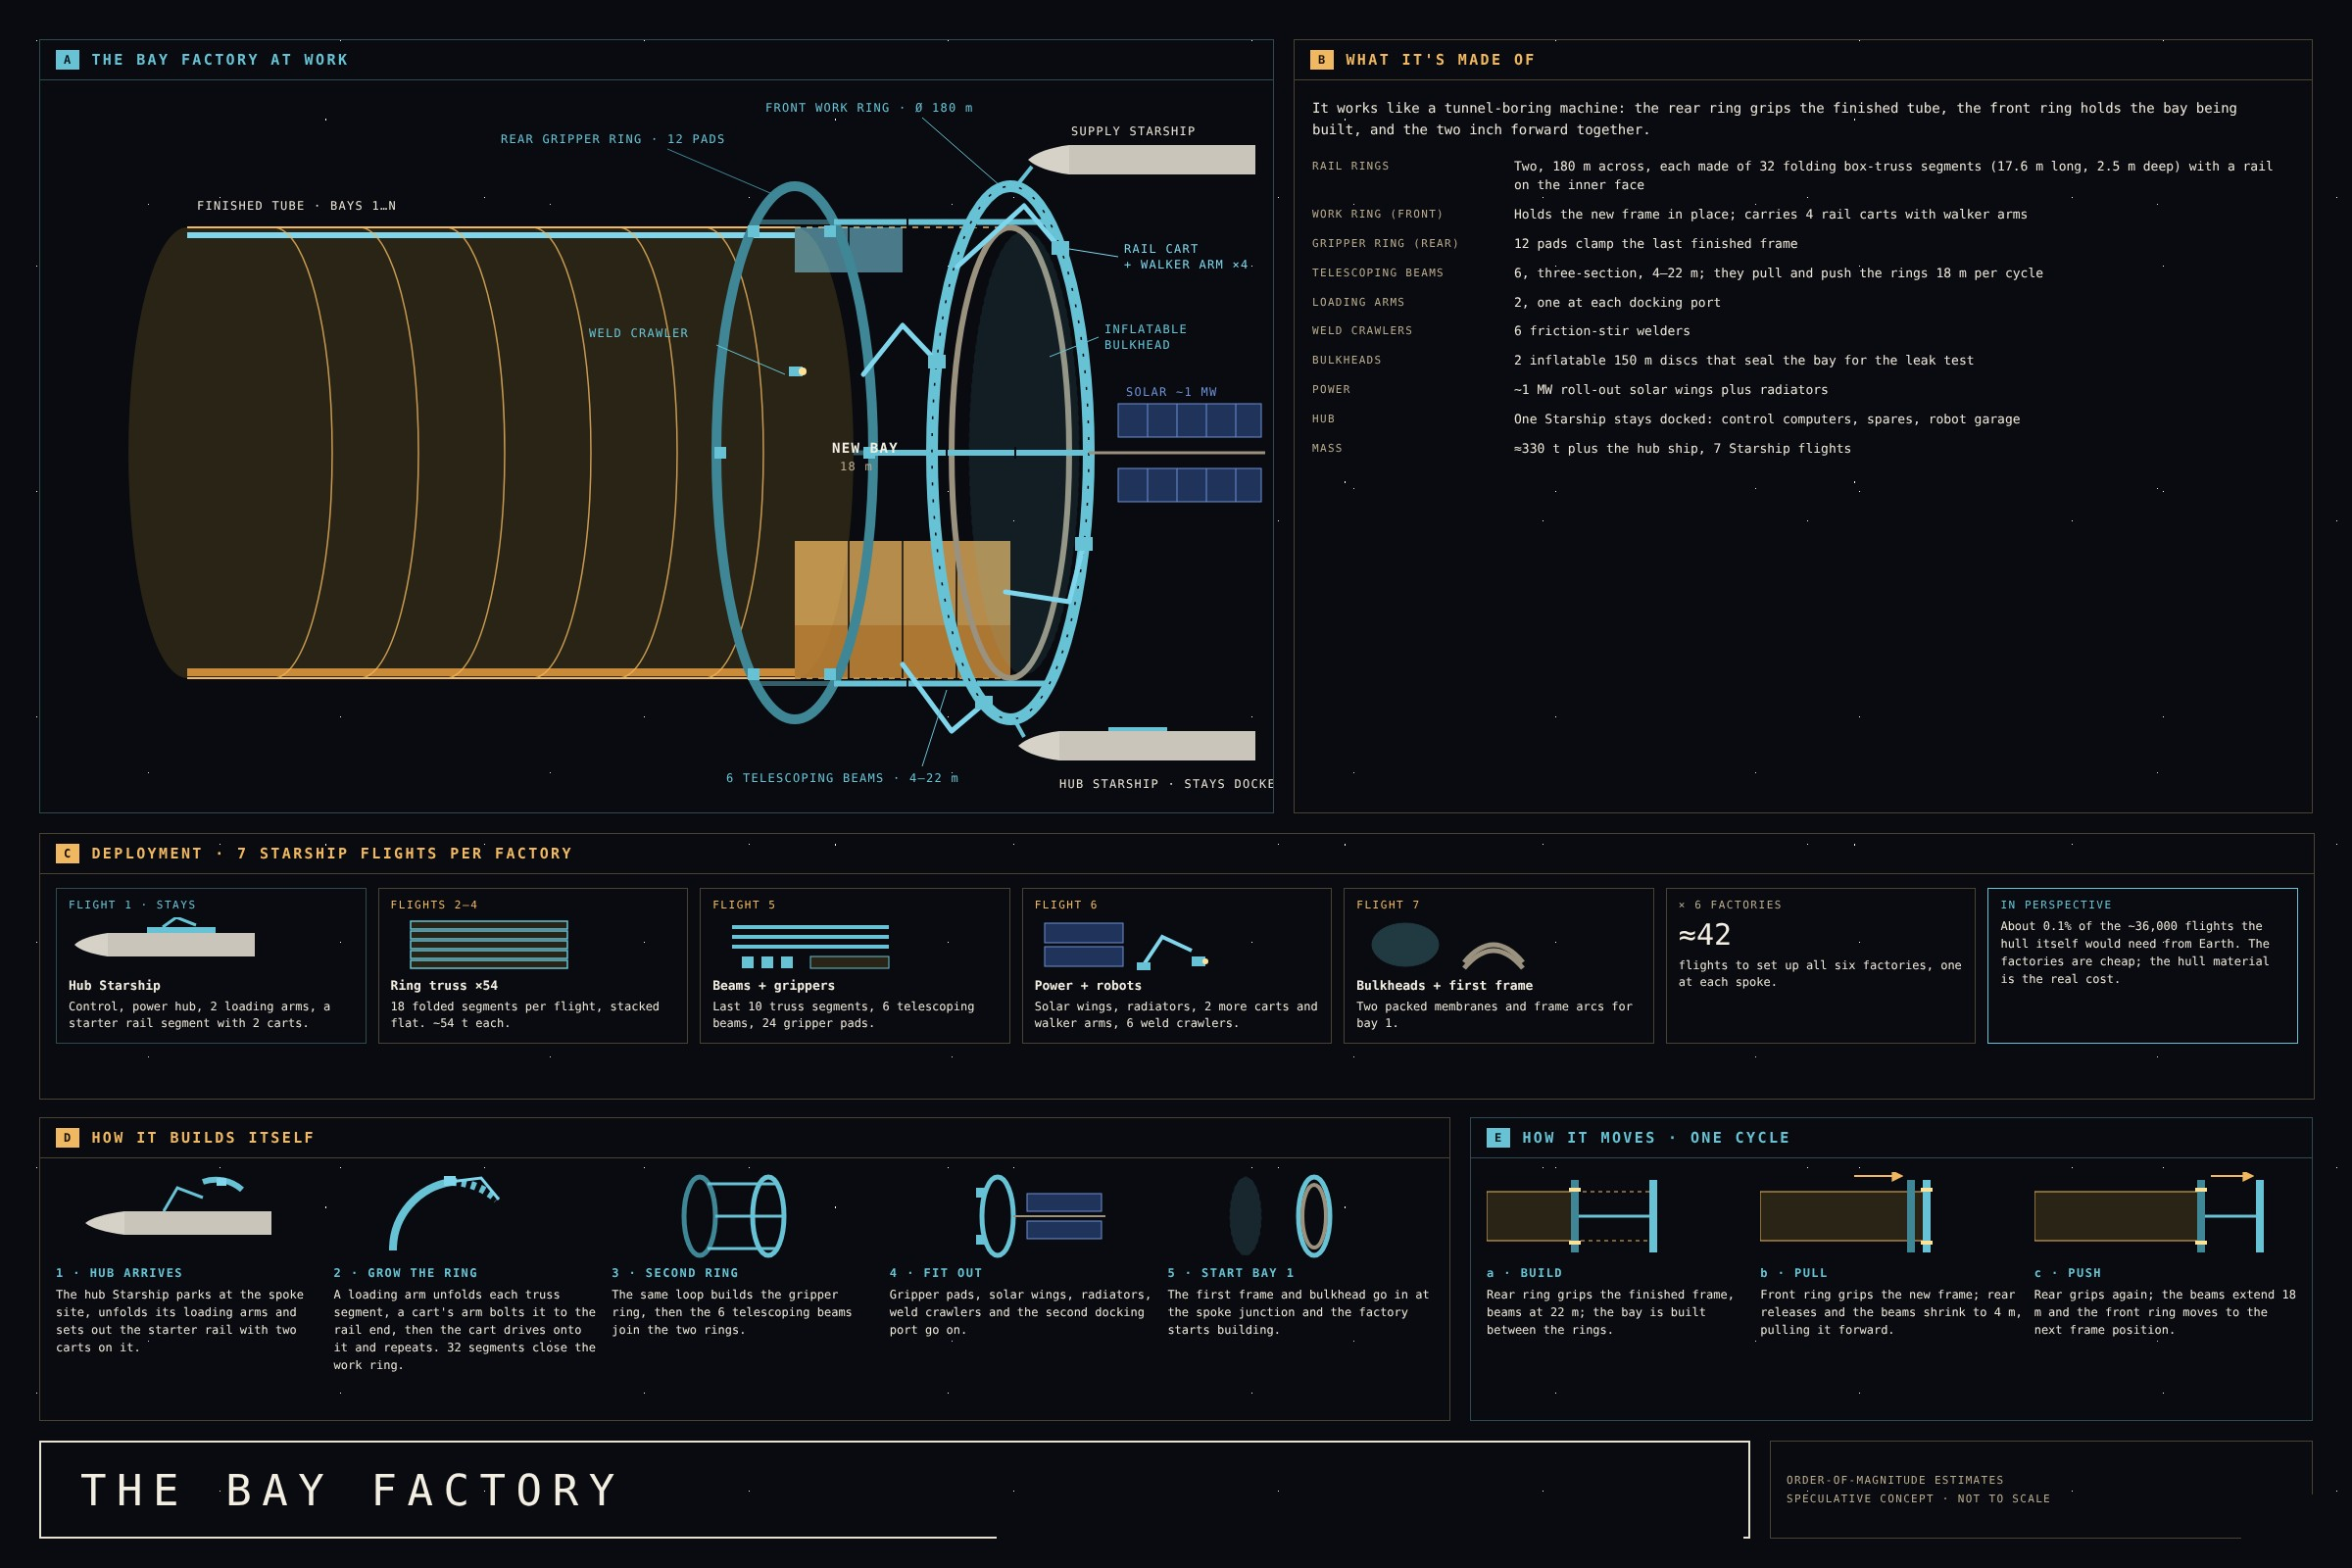
\includegraphics[width=\textwidth]{figures/board-bay-factory.jpg}
  \caption{Design board: the bay factory, its 7 Starship flights and the inchworm cycle.}
\end{figure}

\begin{figure}[H]
  \centering
  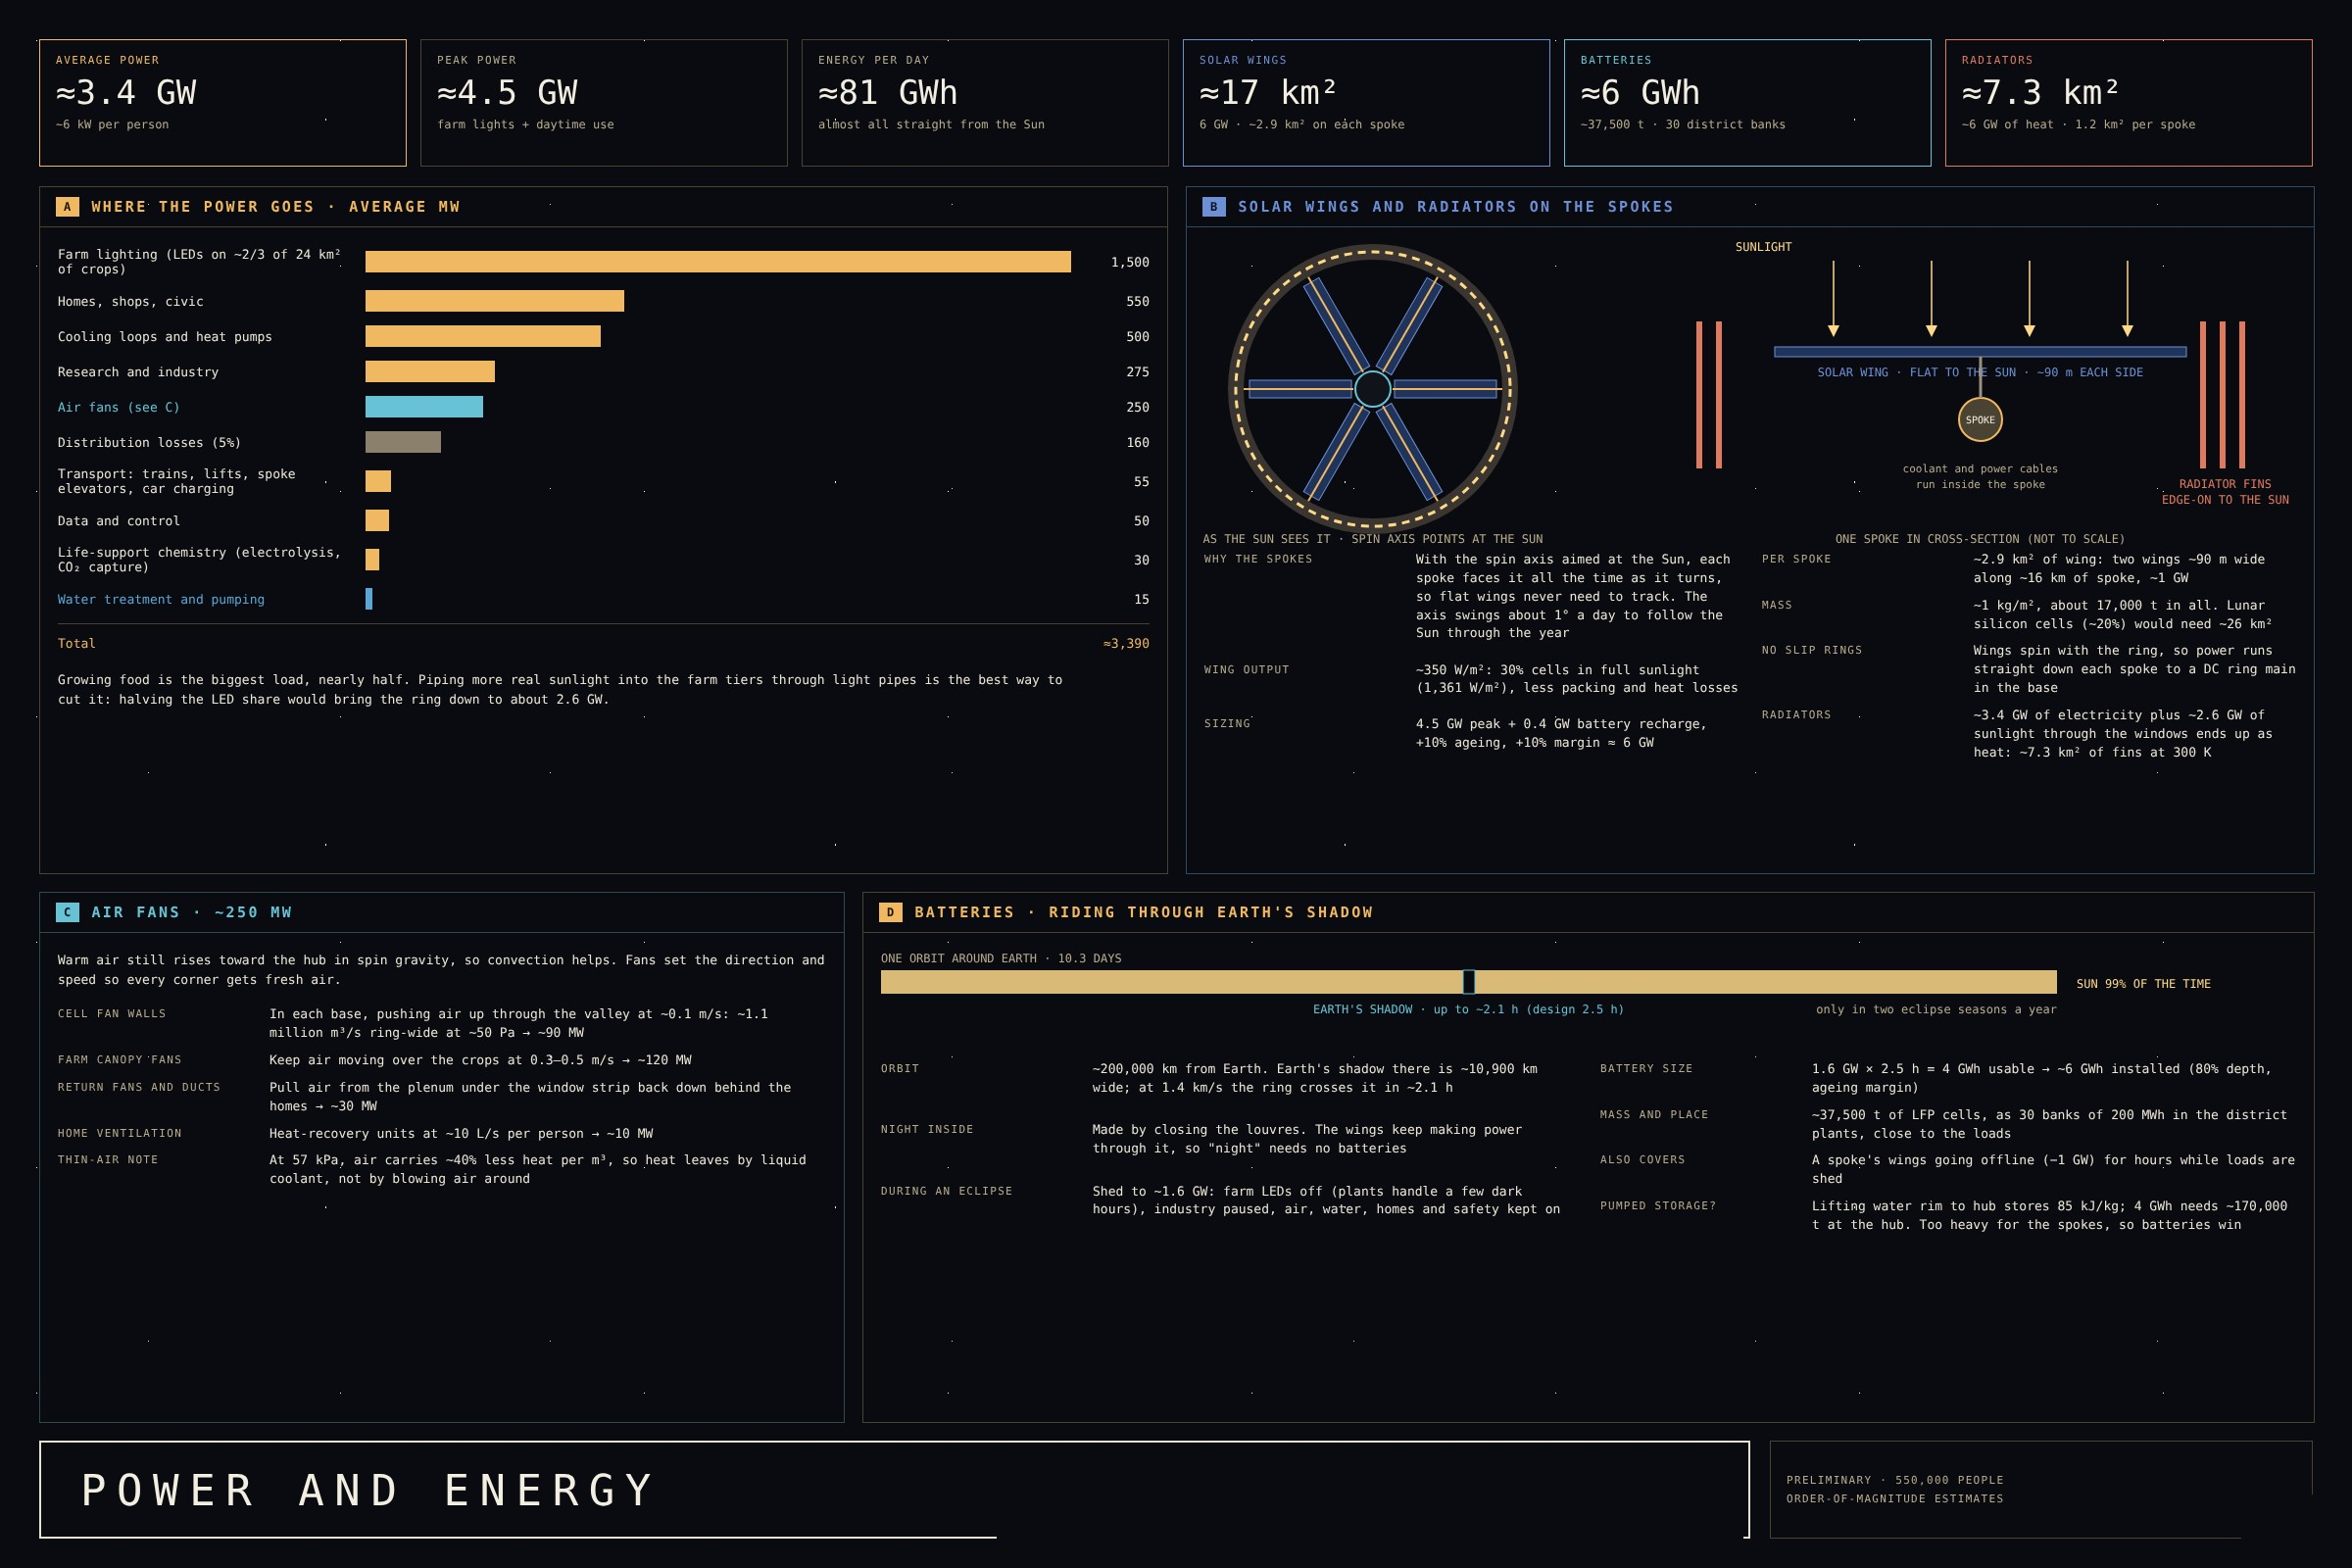
\includegraphics[width=\textwidth]{figures/board-power-and-energy.jpg}
  \caption{Design board: spoke solar wings, batteries and loads, which set the battery tonnage in the launch count.}
\end{figure}
